\chapter{Particle Reconstruction}
\label{sec:reco}

\section{Baselines}

\subsection*{Classification Baseline}\label{app:BDT}

Boosted Decision Trees were chosen as the baseline of comparison for our classification task, due to their popularity with HEP experiments. Decision trees are effective in processing high-level features, performing complex and optimized cut-based classification in the multi-dimensional space of the input quantities. Boosted trees are further able to increase classification accuracy and stability by aggregating the results from multiple trees.

%A BDT still depends on the use of traditional pre-calculated features. Thus, we are able to use the BDT as a stand-in for standard event selection using feature-based cuts.

The features we use for our baseline BDT classification model, introduced in Ref.~\cite{NIPS}, are commonly used to characterize particle showers. One additional feature we added is R9, which measures the largest fraction of energy contained within a 3x3 window in a $(x,y)$ projection of the shower. This quantity provides a measure of the "concentration" of a shower within a small region. For values near 1, the shower is highly collimated within a single region, as in electromagnetic showers. Smaller values are typical of more spread out showers, as for hadronic and multi-prong showers. A comparison of R9 values between photons and neutral pions can be seen in Figure~\ref{fig:R9}, with examples of events with different R9 values being shown in Figure~\ref{fig:R9_examples}. After training, the discriminating power of various features can be seen in Figure~\ref{fig:BDT_ranking}.

\begin{figure}[htbp]
\centering
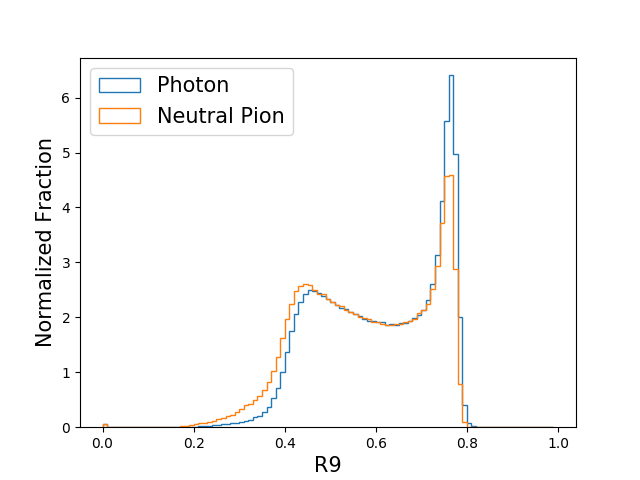
\includegraphics[trim={0 0 0 1cm},clip,width=0.4\textwidth]{images/R9_ratios.png}
\caption{Comparison of R9 distributions between photon and neutral pion events. Photons tend to have more centralized energy deposition.
\label{fig:R9}}
\end{figure}

\begin{figure}[htbp]
\centering
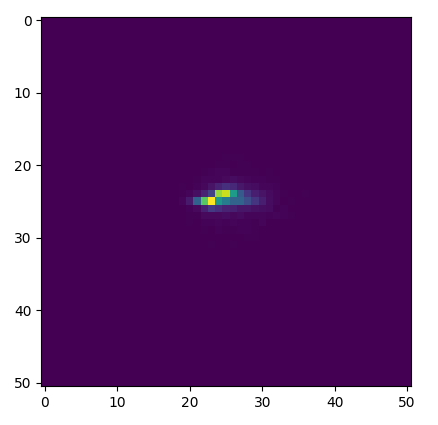
\includegraphics[trim={0 0 0 1cm},clip,width=0.4\textwidth]{images/R9_0p42.png}
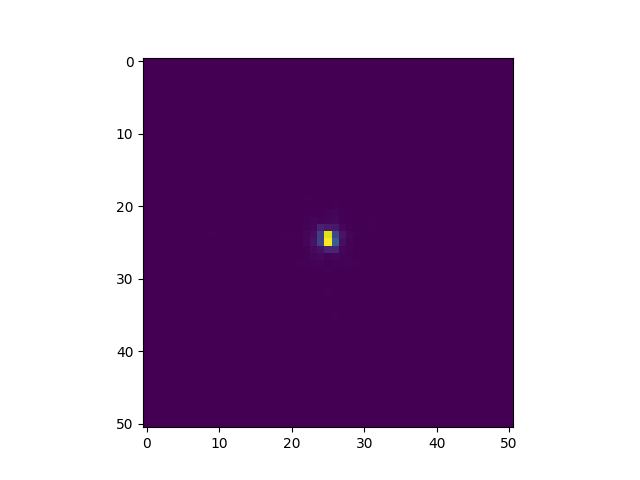
\includegraphics[trim={0 0 0 1cm},clip,width=0.4\textwidth]{images/R9_0p75.png}
\caption{(Top) (x,y) projection of an event with R9=0.42. (Bottom) (x,y) projection of an event with R9=0.75.}
\label{fig:R9_examples}
\end{figure}

\begin{figure}[htbp]
\centering
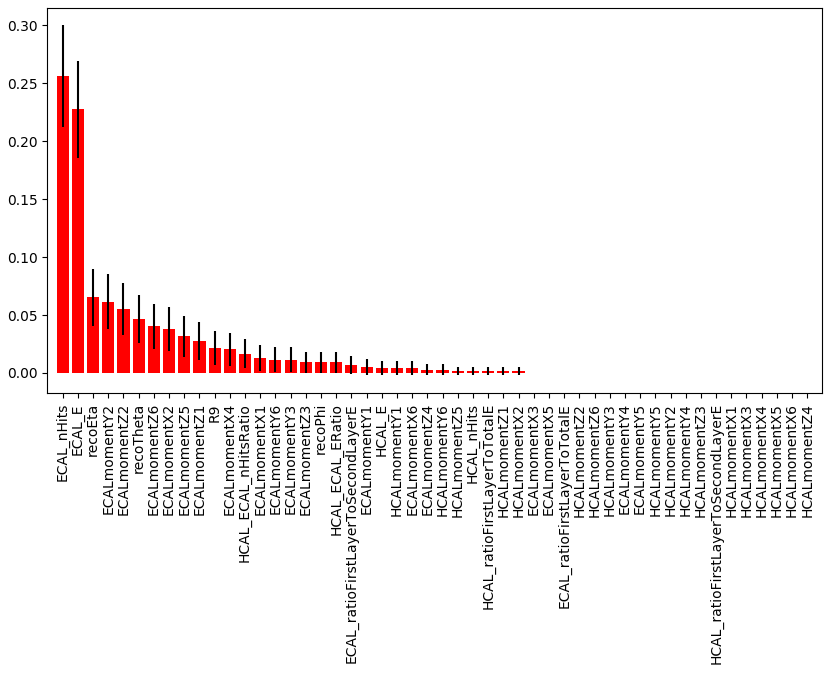
\includegraphics[width=0.43\textwidth]{images/BDT_ranking_fixed.png}
\caption{Feature importances for inputs used in BDT training. Values shown are gini importances~\cite{Breiman}.\label{fig:BDT_ranking}}
\end{figure}

\subsection*{Energy Regression Baseline}\label{app:regression_baseline}

We use linear regression with ECAL and HCAL total energy as one of our baseline methods to compare to machine learning results (seen in Eq.~\ref{eq:linreg}).

\begin{equation}
E = a \cdot E_{ECAL} + b \cdot E_{HCAL} + c
\label{eq:linreg}
\end{equation}

Updated results for each of the particle types are shown in Figure~\ref{fig:reg_linreg}. Each point in the plot represents the mean bias or resolution within an energy bin. In all the resolution plots shown, the points have been fitted with the expected resolution function of Eq.~\ref{eq:res}, and the fitted function is plotted as a line.

\begin{equation}
\frac{\sigma(\Delta E)}{E_{\text{true}}} = \frac{a}{\sqrt{E_{\text{true}}}} \oplus b \oplus \frac{c}{E_{\text{true}}}
\label{eq:res}
\end{equation}

It is already typical for basic ML methods like BDTs to be used for energy regression in the LHC experiments, in cases where the best resolution is critical (e.g., to study $H \rightarrow \gamma\gamma$ decays).  We tried a BDT with a few summary features as input to form an improved baseline for comparing more advanced ML techniques.  The XGBoost package was used in python, with the following hyperparameters.  
\begin{itemize}
\item maximum 1000 iterations, with early stopping if loss doesn't improve on the test set in 10 iterations
\item maximum tree depth of 3
\item minimum child weight of 1 (default)
\item learning rate $\eta = 0.3$ (default)
\end{itemize}
Varying the hyperparameters led to either worse results or negligible changes.

The following features gave good performance for electrons, photons, and \pizero:
\begin{itemize}
\item total ECAL energy
\item total HCAL energy
\item mean $z$ coordinate of the ECAL shower
\end{itemize}

Adding the mean $z$ coordinate to the ECAL and HCAL total energies improved the energy resolution for all energy values, but in particular at high energy. This is shown in Figure~\ref{fig:reg_xgb_ecalmoms} for electrons.

For \chpi, adding the following variables gave an improved result:
\begin{itemize}
\item RMS in the $x$ direction of the ECAL shower
\item RMS in the $(x,y)$ plane of the HCAL shower
\item mean $z$ coordinate of the HCAL shower
\end{itemize}

In addition, for \chpi, around 0.5\% of events were found to have almost no reconstructed energy in the selected calorimeter window.  Including these events adversely affected the algorithm training, so they were removed for all the results shown in this and the following sections. Specifically, the raw ECAL+HCAL energy is required to be at least 30\% of the true generated energy.

%The results of the XGBoost baseline are shown in Fig.~\ref{fig:reg_xgb}, and in Fig.~\ref{fig:reg_xgb_linreg} they are compared to the linear regression results.
The results of the XGBoost baseline are shown in Figure~\ref{fig:reg_xgb_linreg}, where they are compared to linear regression results.
The performance of XGBoost on electrons, photons, and \pizero\ is similar, achieving relative resolutions of about 6--8\% at the lowest energies and 1.0--1.1\% at the highest energies.  Compared to the baseline linear regression, the resolution improves by a factor of about two at low energy and three to four at high energy.  For \chpi, the resolution after XGBoost regression ranges between 20 and 5.4\%, with a relative improvement over linear regression of up to 40\% at high energy.

%\begin{figure}[htbp]
%\centering
%\includegraphics[width=0.38\textwidth]{images/bias_vs_E_allparts_xgb_zoom.pdf}
%\includegraphics[width=0.38\textwidth]{images/res_vs_E_allparts_xgb_fits.pdf}
%\caption{Bias (top) and resolution (bottom) as a function of true energy for XGBoost regression predictions of particle energy for the different particle types.  
%}
%\label{fig:reg_xgb}
%\end{figure}

One drawback of using a BDT algorithm in a real-world setting is that it can not be used for energy values outside the range of the training set. That is, most tree algorithms do not perform extrapolation. This is an inherent disadvantage of the BDT when compared with the neural networks we present in this paper.

\begin{figure}[htbp]
\centering
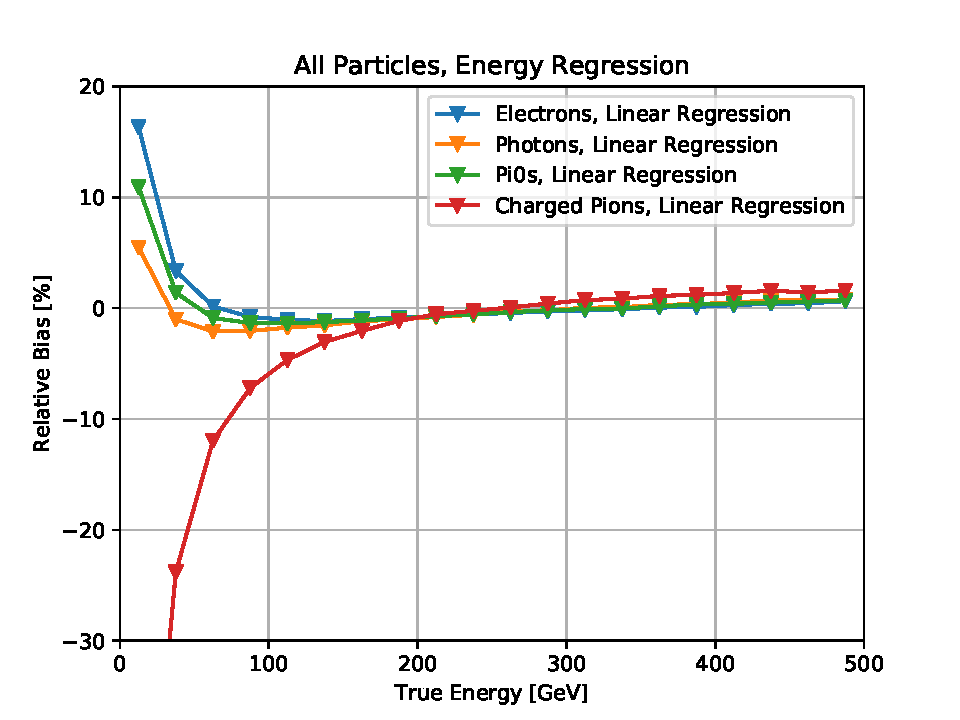
\includegraphics[width=0.38\textwidth]{images/bias_vs_E_allparts_linreg.pdf}
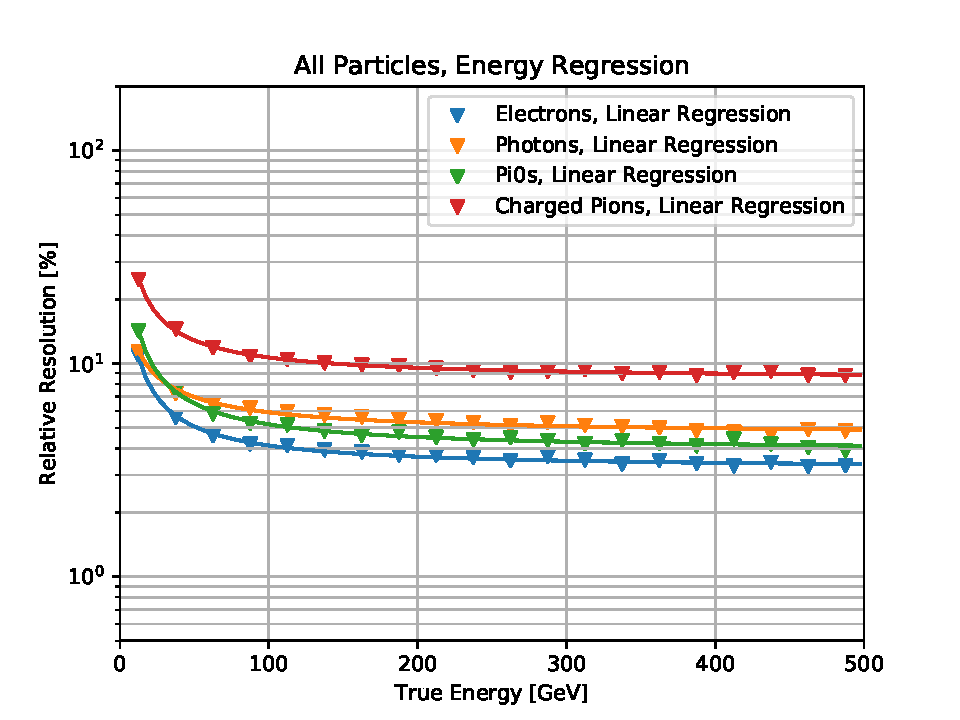
\includegraphics[width=0.38\textwidth]{images/res_vs_E_allparts_linreg_fits.pdf}
\caption{Bias (top) and resolution (bottom) as a function of true energy for linear regression predictions of particle energy for the different particle types, trained on fixed-angle samples. \label{fig:reg_linreg}}
\end{figure}

\begin{figure}[htbp]
\centering
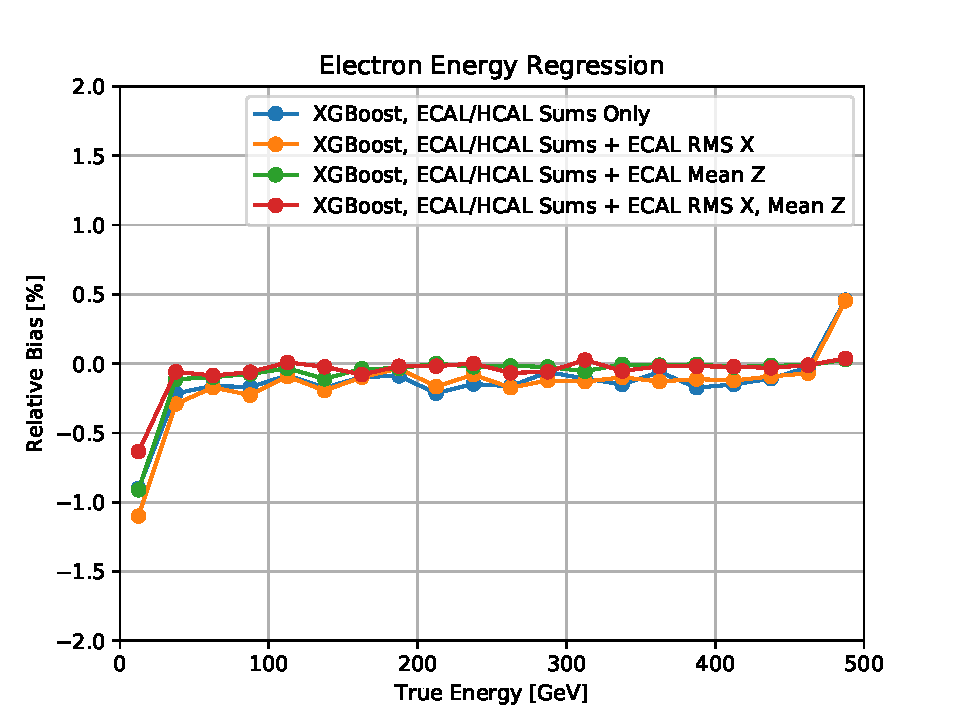
\includegraphics[width=0.38\textwidth]{images/bias_vs_E_EleFixed_xgb_ecalmoms_zoom.pdf}
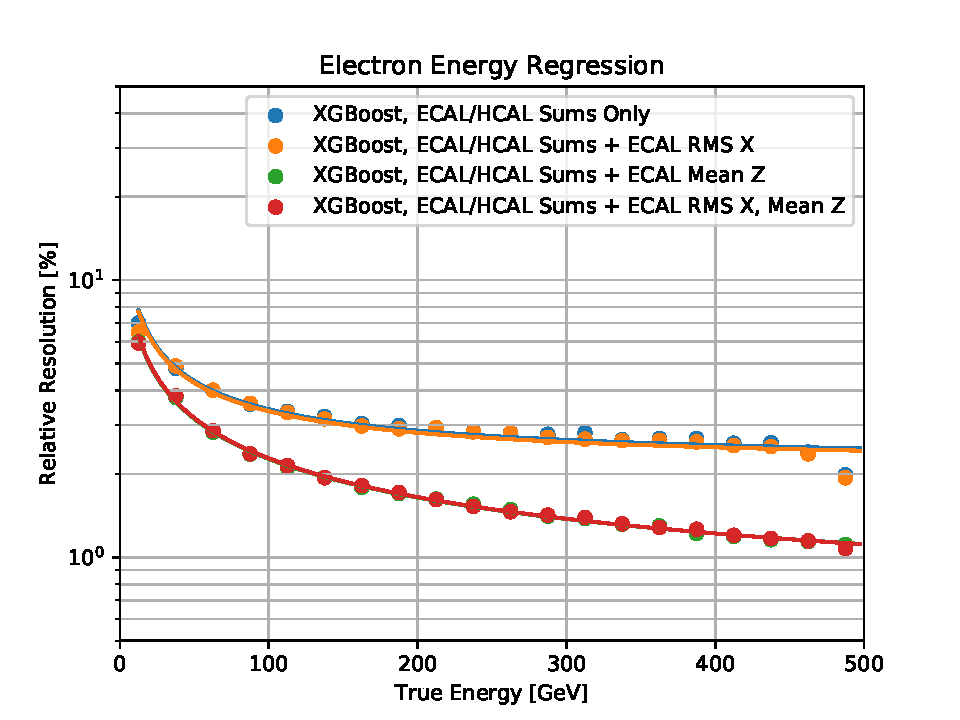
\includegraphics[width=0.38\textwidth]{images/res_vs_E_EleFixed_xgb_ecalmoms_fits.pdf}
\caption{Bias (top) and resolution (bottom) as a function of true energy for the XGBoost regression predictions of particle energy, using different input features for electrons.\label{fig:reg_xgb_ecalmoms}}
\end{figure}

\begin{figure}[htbp]
\centering
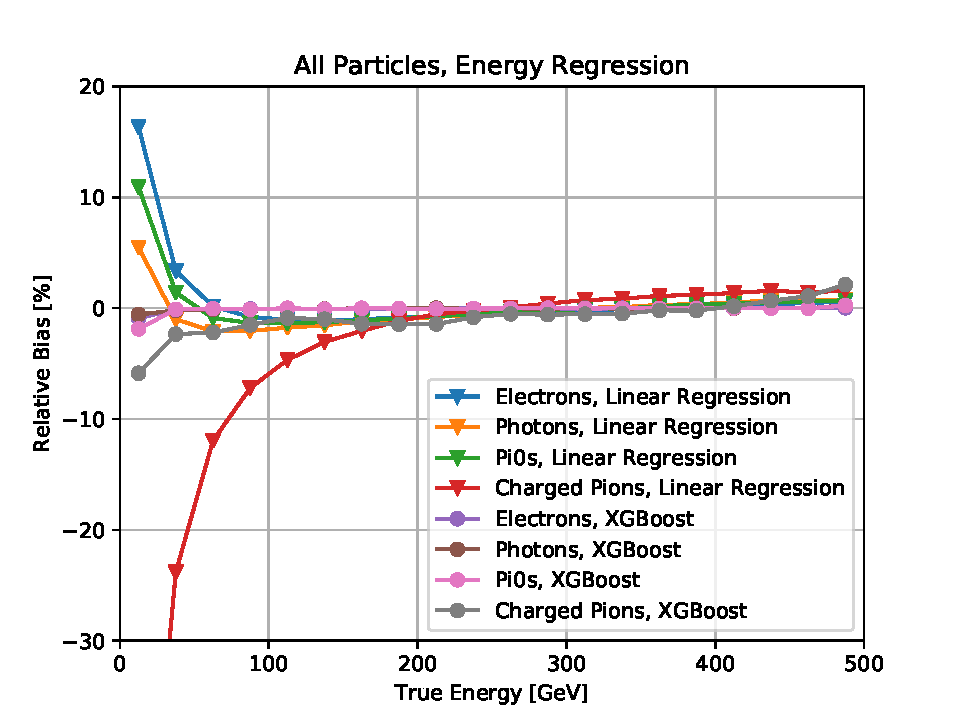
\includegraphics[width=0.38\textwidth]{images/bias_vs_E_allparts_linreg_xgb.pdf}
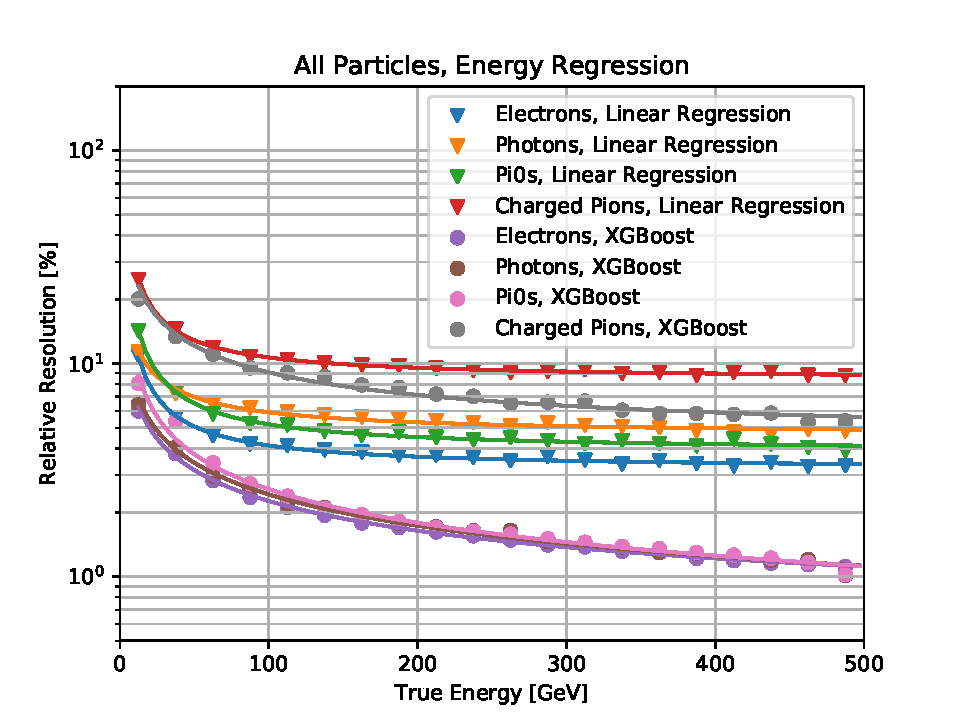
\includegraphics[width=0.38\textwidth]{images/res_vs_E_allparts_linreg_xgb_fits.pdf}
\caption{Bias (top) and resolution (bottom) as a function of true energy for linear regression and XGBoost  predictions of particle energy for the different particle types.\label{fig:reg_xgb_linreg}}
\end{figure}

\section{Classification}

This section describes the use of a deep neural network to accomplish an end-to-end particle reconstruction task. The model consists of a neural architecture which simultaneously performs both particle classification and energy regression. This combined network is trained using the ECAL and HCAL cell arrays as well as the total ECAL energy and total HCAL energy as inputs. The training loss function is written as the sum of a binary cross entropy for particle identification and a mean-square error loss for energy regression. Through experimentation, we found that multiplying the energy component of the loss function by a factor of 200 gave the best results, as it was easier to quickly achieve low loss values for energy regression.

We compare three different architectures for our reconstruction model, each trained using calorimeter cell-level information as inputs:
\begin{itemize}
\item A dense (i.e, fully connected) neural network (DNN).
\item A 3D convolutional network (CNN).
\item A network based on GoogLeNet (GN)~\cite{GoogLeNet}, using layers of inception modules.
\end{itemize}

In order to compare the model performance to a typical state-of-the-art particle reconstruction algorithm, we also consider the following alternatives:
\begin{itemize}
    \item A feature-based BDT (see Appendix~\ref{app:BDT}) for the classification task.
    \item A linear regression for the regression task.
    \item A BDT for the regression task (for more info on regression baselines see Appendix~\ref{app:regression_baseline}).
\end{itemize}

In a previous study~\cite{NIPS}, we compared the classification accuracy obtained with a neural model taking as input the energy cells, a feature-based neural models, and a feature-based BDTs. In that context, we demonstrated that feature-based BDTs and neural networks perform equally well, and are both equally capable of correctly classify particles from a small set of calculated features. 
%Increases in classification accuracy are mostly due to the neural architecture's ability to extract meaning from a much larger input dataset, the calorimeter cell-level energy information. For this reason, w
We do not compare feature-based neural networks in this paper, and use feature-based BDTs to represent the current state-of-the-art classification algorithms.

\subsection{Deep Network Models}

The three ML models take as input the ECAL and HCAL 3D energy arrays of the REC dataset (see Section~\ref{sec:data}), together with the total energies recorded in ECAL and in HCAL (i.e., the sum of the values stored in the 3D arrays), as well as the estimated $\phi$ and $\eta$ angles of the incoming particle, calculated using the collision origin and the barycenter of the event. The architecture of each model is defined with a number of floating parameters (e.g. number of hidden layers), which are refined through a hyperparameter optimization, as described in Section~\ref{sec:hpscan}. Each model returns three numbers. After applying a softmax activation, two of these elements are interpreted as the classification probabilities of the current two-class problem. The third output is interpreted as the energy of the particle.

Here we describe in detail the three model architectures:

\begin{itemize}
    \item In the DNN model we first flatten our ECAL and HCAL inputs into 1D arrays. We then concatenate these array along with the total ECAL energy, total HCAL energy, estimated $\phi$, and estimated $\eta$, for an array of total size $25 \times 25 \times 25 + 11 \times 11 \times 60 + 4 = 22889$ inputs. This array is fed as input to the first layer of the DNN, followed by a number of hidden layers each followed by a ReLU activation function and a dropout layer. The number of neurons per hidden layer and the dropout probability are identical for each relevant layer. The number of hidden layers, number of hidden neurons per layer, and dropout rate are hyperparameters, tuned as described in the next session.  Finally, we take the output from the last dropout layer, append the total energies and estimated angles again, and feed the concatenated array into a final hidden layer, which results in a three-element output. 
    \item The CNN architecture consists of one 3D convolutional layer for each of the ECAL and HCAL inputs, each followed by a ReLU activation function and a max pooling layer of kernel size $2 \times 2 \times 2$. The number of filters and the kernel size in the ECAL convolutional layer are treated as optimized hyperparameter (see next session). The HCAL layer is fixed at 3 filters with a kernel size of $2 \times 2 \times 6$. The two outputs are then flattened and concatenated along with the total ECAL and HCAL energies, as well as the estimated $\phi$ and $\eta$ coordinates of the incoming particle. The resulting 1D array is passed to a sequence of dense layers each followed by a ReLU activation function and dropout layer, as in the DNN model. The number of hidden layers and the number of neurons on each layer are considered as hyperparameters to be optimized. The output layer consists of three numbers, as for the DNN model. We found that adding additional convolutional layers to this model beyond the first had little impact on performance. This may be because a single layer is already able to capture important information about localized shower structure, and reduces the dimensionality of the event enough where a densely connected net is able to do the rest.
    \item The third model uses elements of the GoogLeNet~\cite{GoogLeNet} architecture. This network processes the ECAL input array with a 3D convolutional layer with 192 filters, a kernel size of 3 in all directions, and a stride size of 1. The result is batch-normalized and sent through a ReLU activation function. This is followed by a series of inception and MaxPool~\cite{conv} layers of various sizes, with the full architecture described in Appendix~\ref{app:GoogLeNet}. The output of this sequence is concatenated to the total ECAL energy, the total HCAL energy, the estimated $\phi$ and $\eta$ coordinates, and passed to a series of dense layers like in the DNN architecture, to return the final three outputs. The number of neurons in the final dense hidden layer is the only architecture-related hyperparameter for the GN model. Due to practical limitations imposed by memory constraints, this model does not take the HCAL 3D array as input. This limitation has a small impact on the model performance, since the ECAL array carries the majority of the relevant information for the problems at hand (see Appendix~\ref{app:classification_HCAL}).
\end{itemize}

On all models, the regression task is facilitated by using skip connections to directly append the input total ECAL and HCAL energies to the last layer. The impact of this architecture choice on regression performance is described in Appendix~\ref{app:skip_connections}. In addition to using total energies, we also tested the possibility of using 2D projections of the input energy arrays, summing along the $z$ dimension (detector depth). This choice resulted in worse performance (see Appendix~\ref{app:z_sum_regression}) and was discarded.

\subsection{Hyperparameter Scans}
\label{sec:hpscan}

In order to determine the best architectures for the end-to-end reconstruction models, we scanned over a hyperparameter space for each architecture. Learning rate and decay rate were additional hyperparameters for each architecture. For simplicity, we used classification accuracy for the $\gamma$ vs. $\pi^0$ problem as a metric to determine the overall best hyperparameter set for each architecture. This is because a model optimized for this task was found to generate good results for the other three tasks as well, and because $\gamma$ vs. $\pi^0$ classification was found to be the most difficult problem.

Training was performed at each hyperparameter point ten times, in order to obtain an estimate of the uncertainty associated with each quoted performance value. For each scan point, the DNN and CNN architectures trained on 400,000 events, using another sample of 400,000 events for testing. DNN and CNN scan points trained for three epochs each, taking about seven hours each. GN trained on 100,000 events and tested on another 100,000. Due to a higher training time, each GN scan point only trained for a single epoch, taking about twenty hours.

For CNN and DNN training, we used batches of 1,000 events when training. However, due to GPU memory limitations, we could not do the same with GN. Instead, we split each batch into 100 minibatches of ten events each. A single minibatch was loaded on the GPU at a time, and gradients were added up after back-propagation. We waited until after each batch was fully calculated to update network weights using the combined gradients.

The best settings were found to be as follows:
\begin{itemize}
    \item For DNN, 4 hidden layers, 512 neurons per hidden layer, a learning rate of 0.0002, decay rate of 0, and a dropout probability of 0.04.
    \item For CNN, 4 hidden layers and 512 neurons per hidden layer, a learning rate of 0.0004, decay rate of 0, a dropout probability of 0.12, 6 ECAL filters with a kernel size of $6 \times 6 \times 6$.
    \item For GN, 1024 neurons in the hidden layer, 0.0001 learning rate, and 0.01 decay rate. 
\end{itemize}
%For CNN and GN, a very mild dependence on the number of neurons per hidden layer is observed. 

\begin{figure*}[htbp]
\centering
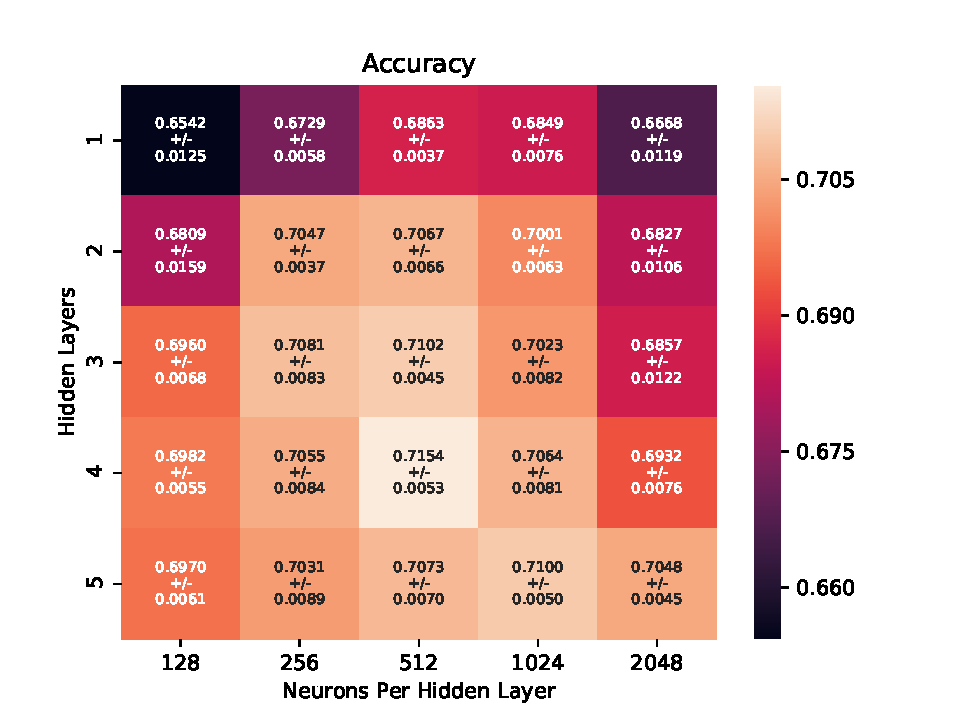
\includegraphics[width=0.45\textwidth]{images/DNN_hl_nhl}
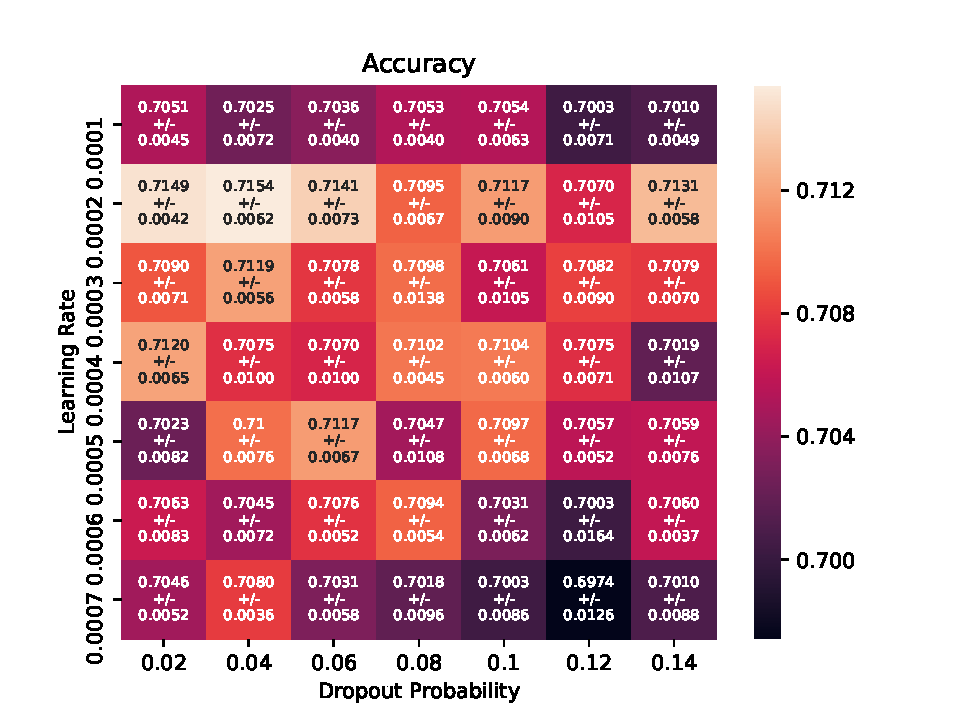
\includegraphics[width=0.45\textwidth]{images/DNN_lr_dp} \\
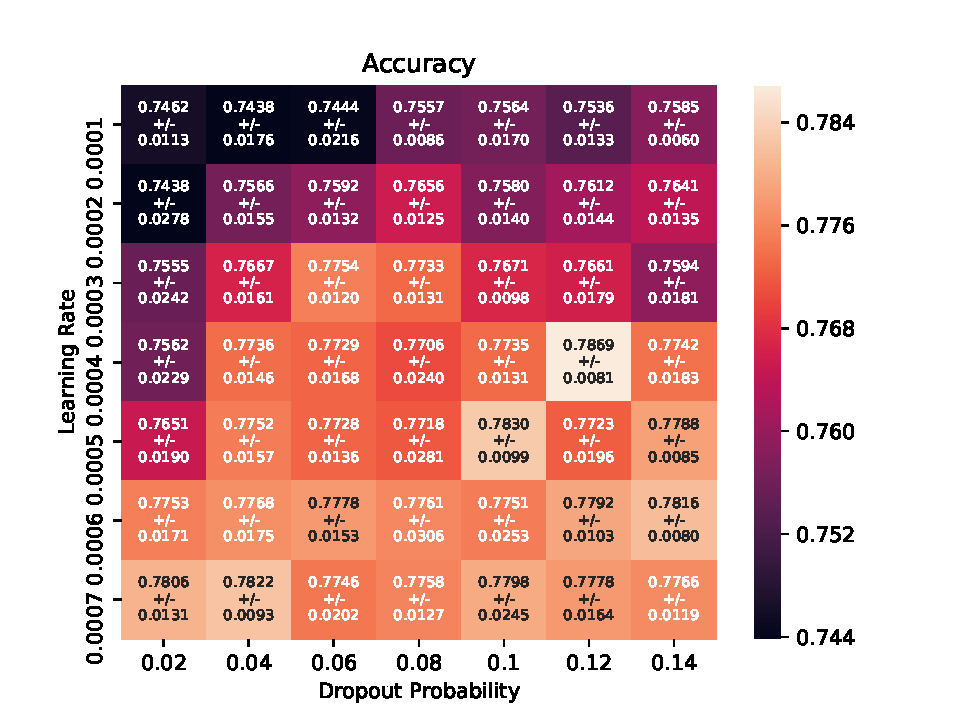
\includegraphics[width=0.45\textwidth]{images/CNN_lr_dp}
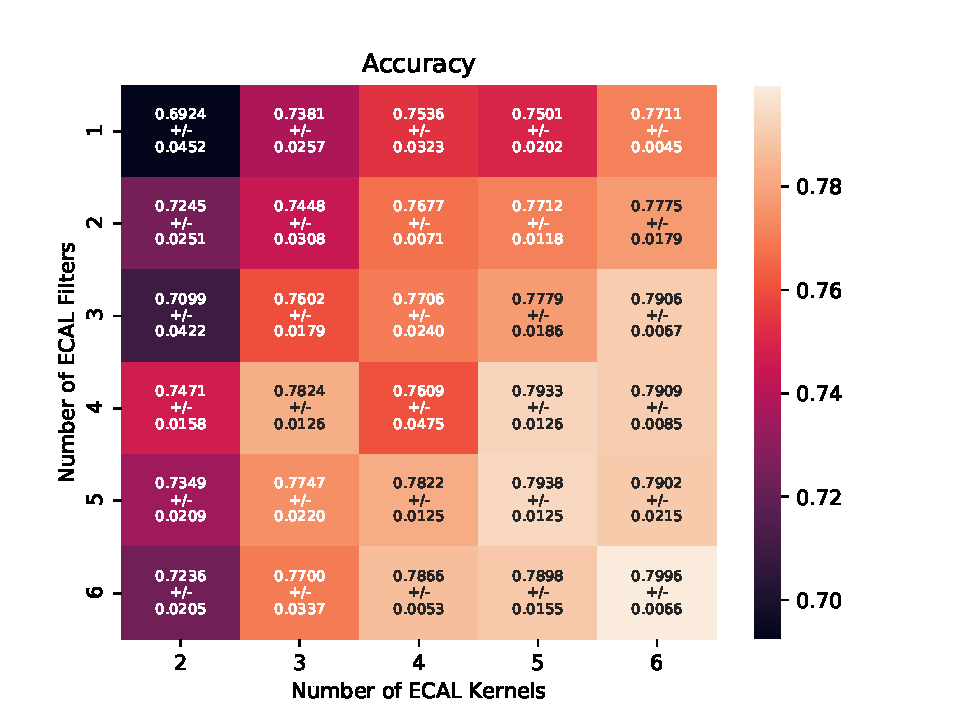
\includegraphics[width=0.45\textwidth]{images/CNN_nECALfilt_nECALkern} \\
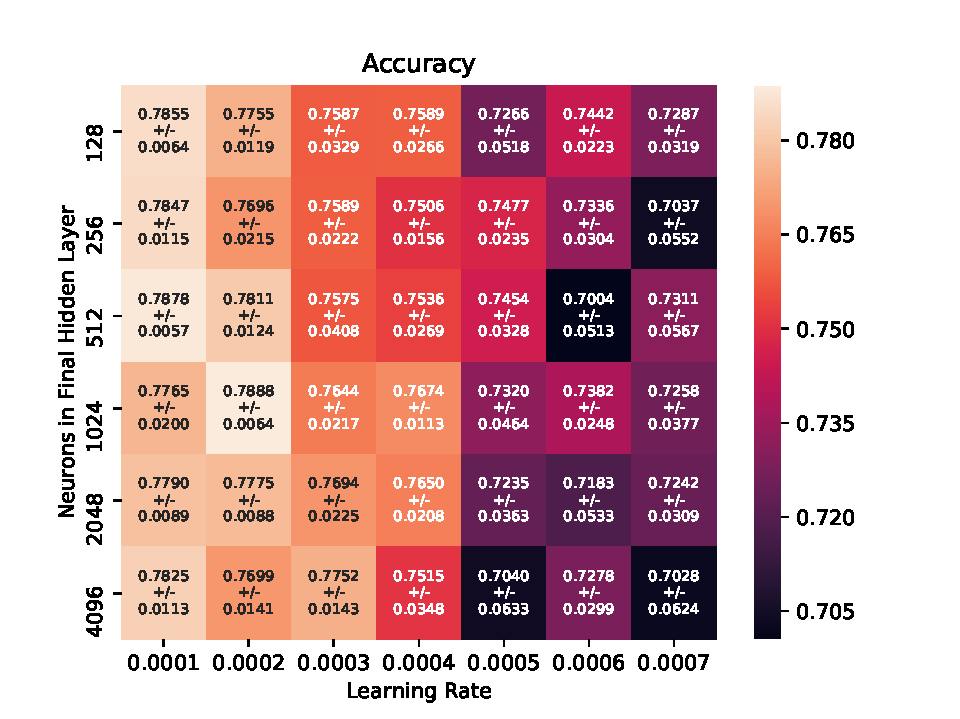
\includegraphics[width=0.45\textwidth]{images/GN_nhl_lr}
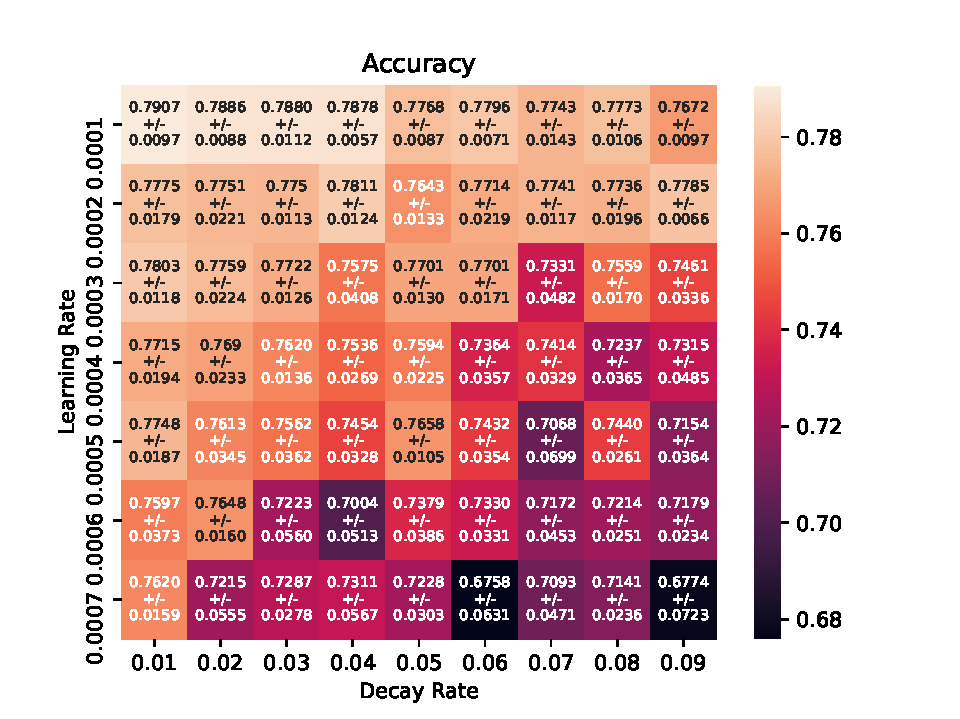
\includegraphics[width=0.45\textwidth]{images/GN_lr_dr}
\caption{Selected hyperparameter scan results for DNN (top), CNN (center), and the GoogLeNet-based architecture (bottom). In each figure, the classification accuracy is displayed as a function of the hyperparameters reported on the two axes.}
\label{fig:scan_hyperparameter}
\end{figure*}

The DNN, CNN, and GN-based models had 9823774 ($\sim$10M), 3003692 ($\sim$3M), and 14956286 ($\sim$15M) trainable parameters respectively after the hyperparameter scans.

Selected hyperparameter scan slices are shown in Figure~\ref{fig:scan_hyperparameter}. 
These 2D scans were obtained setting all values besides the two under consideration (i.e., those on the axes) to be fixed at default values: a dropout rate of 0.08, a learning rate of 0.0004, a decay rate of 0.04, three dense layers for CNN and DNN, and 512 neurons per hidden layer. For GN, the default number of ECAL filters was 3, with a kernel size of 4.
%An ECAL window size of 25 was used in all instances, to allow fair comparison between DNN, CNN, and GN, as larger ECAL sizes posed a memory problem when training GN.

After performing the hyperparameter scan, we trained each architecture using its optimal hyperparameters for a greater number of epochs. The evolution of the training and validation accuracy as a function of the batch number for these extended trainings is shown in Figure~\ref{fig:training_curves_comparison_gamma_pi0}.

\begin{figure}[htbp]
\centering
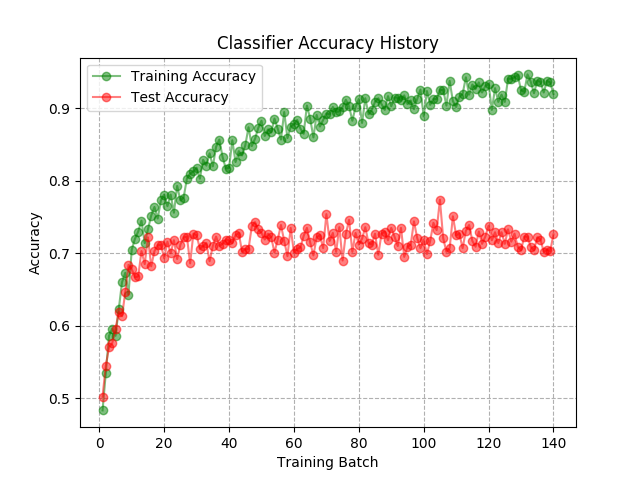
\includegraphics[width=0.42\textwidth]{images/DNN_accuracy_batches_long}
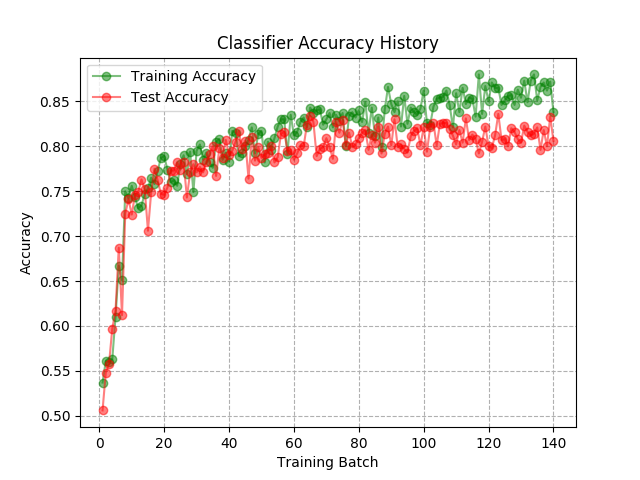
\includegraphics[width=0.42\textwidth]{images/CNN_accuracy_batches_long}
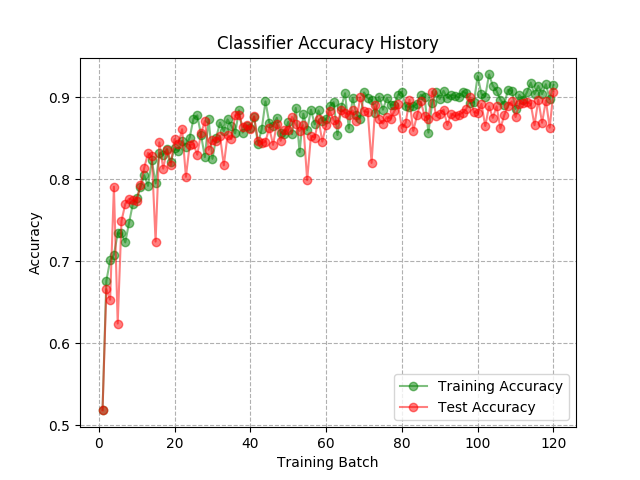
\includegraphics[width=0.42\textwidth]{images/GN_accuracy_batches_long}
\caption{Training curves for best DNN (top), CNN (middle), and GoogLeNet (bottom) hyperparameters, trained on variable-angle $\gamma$/$\pi^0$ samples. We see that the DNN over-trains quickly and saturates at a relatively low accuracy, while the CNN takes longer to over-train and reaches a higher accuracy, and GoogLeNet performs best of all. Each 400 batches corresponds to a single epoch.}
\label{fig:training_curves_comparison_gamma_pi0}
\end{figure}

\subsection{Results}

We apply the best architectures described in the previous section separately to our electron vs. charged pion and photon vs. neutral pion reconstruction problems.

\subsubsection{Classification Performance}
\label{sec:classification}

Figure~\ref{fig:architectures_ROC_comparisons} shows ROC curve comparisons for the two classification tasks. As expected, the electron vs. charged pion classification problem was found to be a simple task, resulting in an area under the curve (AUC) close to $100\%$. For a baseline comparison, the curve obtained for a BDT (see Appendix~\ref{app:BDT}) is also shown. This BDT was optimized using the {\it scikit-optimize} package~\cite{skopt}, and was trained using high-level features computed from the raw 3D arrays. It represents the performance of current (non-deep-learning) ML approaches on these problems.

\begin{figure}[htbp]
\centering
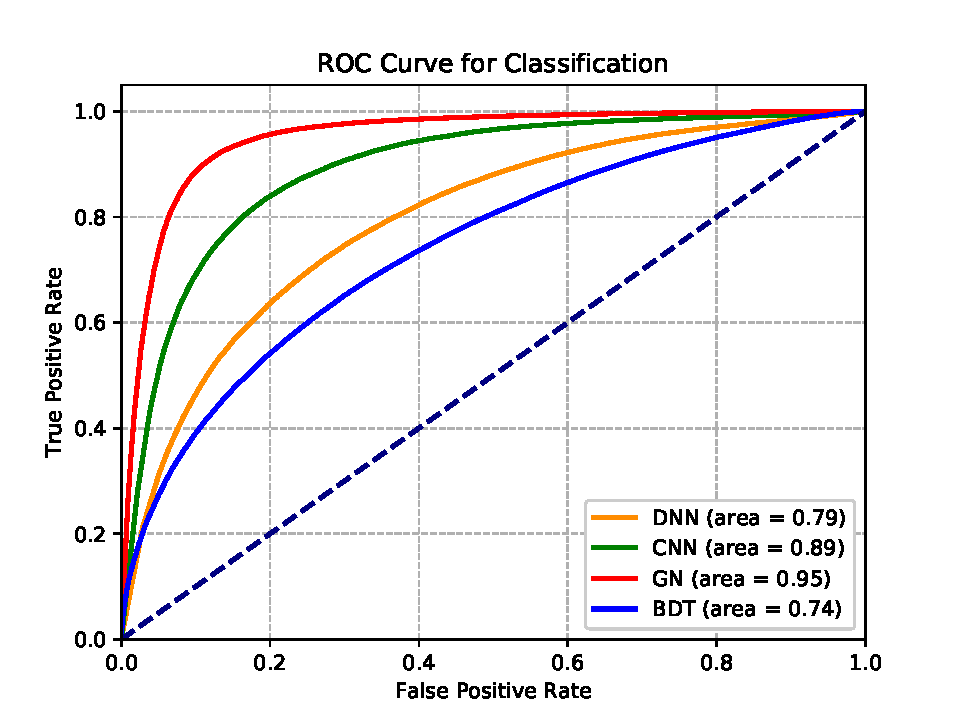
\includegraphics[width=0.45\textwidth]{images/architectures_ROC_comparison_gamma_pi0_long}
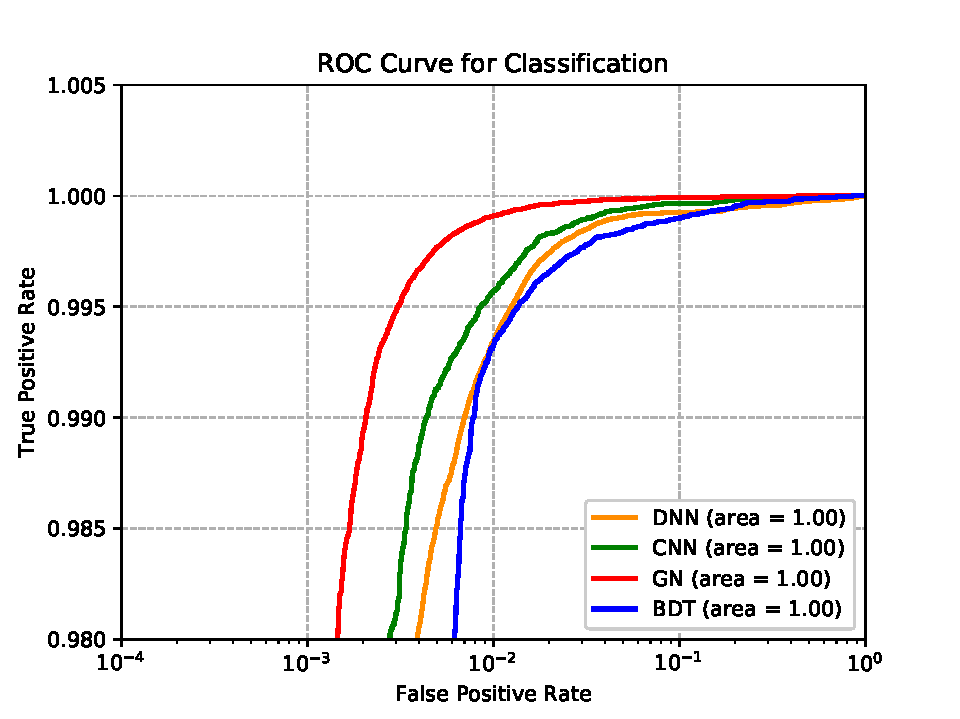
\includegraphics[width=0.45\textwidth]{images/architectures_ROC_comparison_ele_chpi_xlog}
\caption{ROC curve comparisons for $\gamma$ vs. $\pi^0$ (top) and $e$ vs. $\pi^\pm$ (bottom) classification using DNN, CNN, BDT, and GoogLeNet (GN). Samples include particle energies from 2 to 500 GeV, and an inclusive $\eta$ range.}
\label{fig:architectures_ROC_comparisons}
\end{figure}

Our deep learning models outperform the BDT, with the GN reaching the best classification performance on both problems. Figure~\ref{fig:accuracy_bins} shows the best-model performance as a function of the energy and $\eta$ of the incoming particle, for the photon vs. neutral pion and the electron vs. charged pion problems. These figures show that classification accuracy is maintained over a wide range of particle energies and angles. The models appear to perform a bit worse at higher energies for the photon vs. neutral pion case, due to the fact that the pion to two photon decay becomes increasingly collimated at higher energies. Similarly, the performance is slightly worse when particles impact the detector perpendicularly than when they enter at a wide angle, because the shower cross section on the calorimeter inner surface is reduced at $90^{\mathrm o}$, making it harder to distinguish shower features.

\begin{figure*}[htbp]
\centering
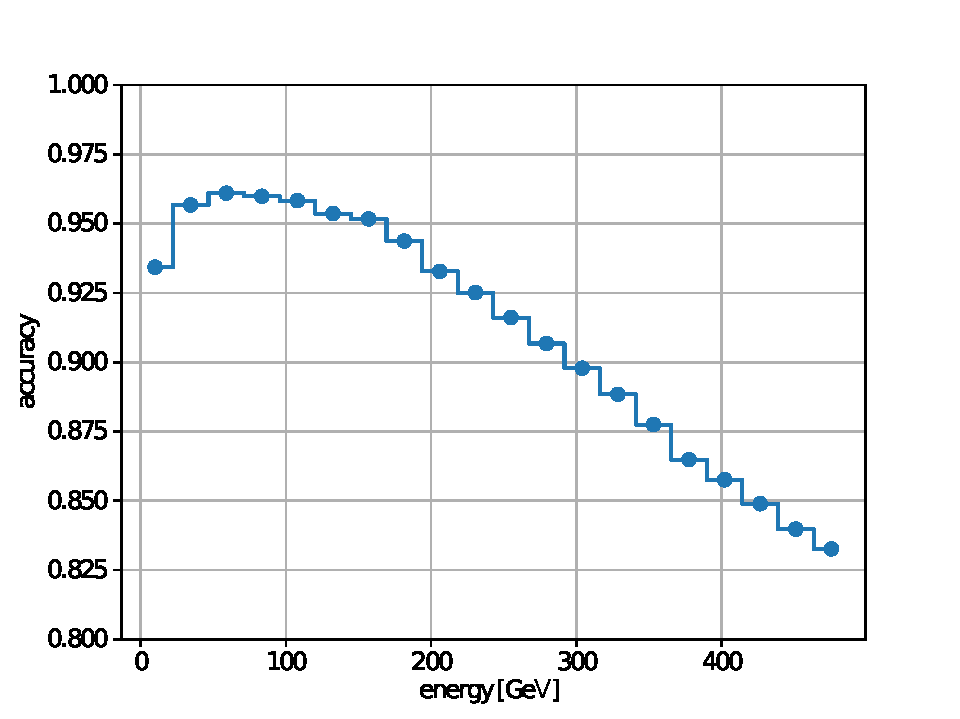
\includegraphics[width=0.45\textwidth]{images/gamma_pi0_accuracy_energy_bins.pdf}
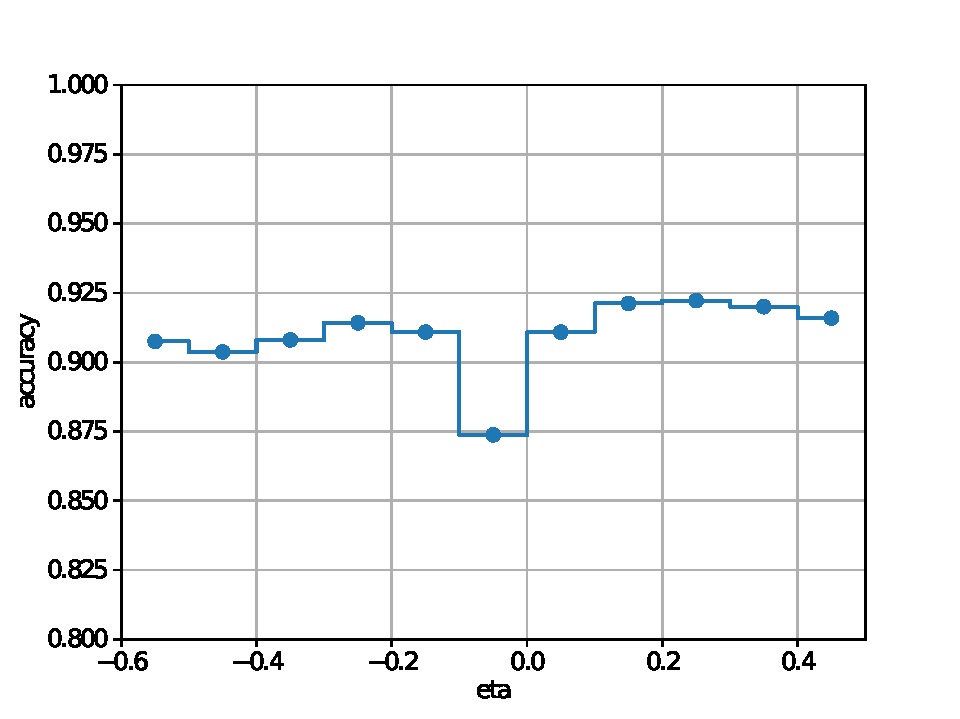
\includegraphics[width=0.45\textwidth]{images/gamma_pi0_accuracy_eta_bins.pdf} \\
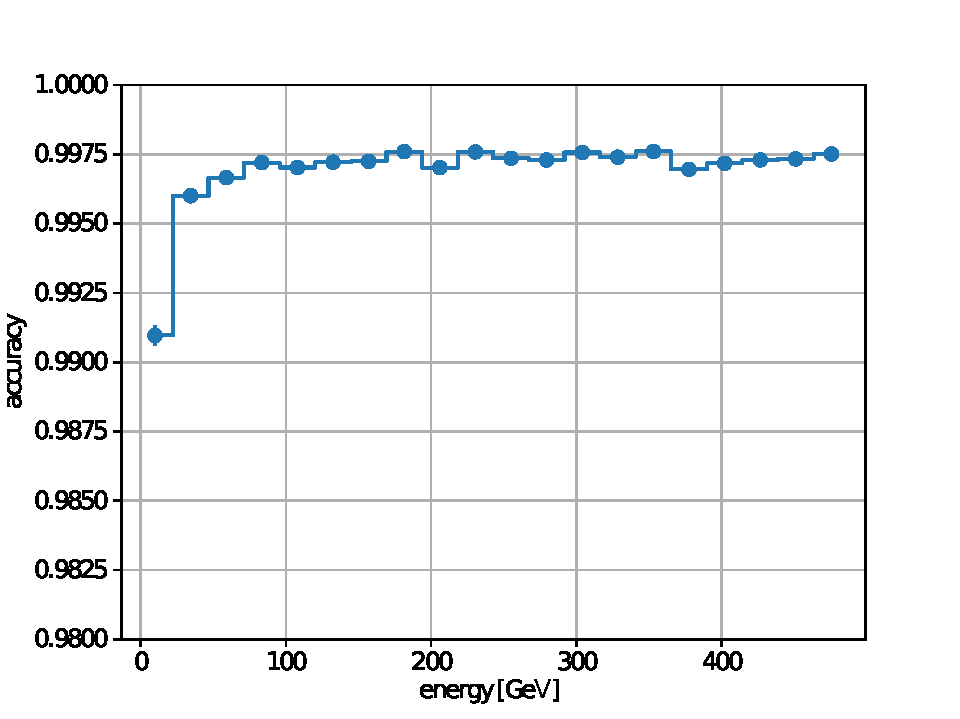
\includegraphics[width=0.45\textwidth]{images/ele_chpi_accuracy_energy_bins.pdf}
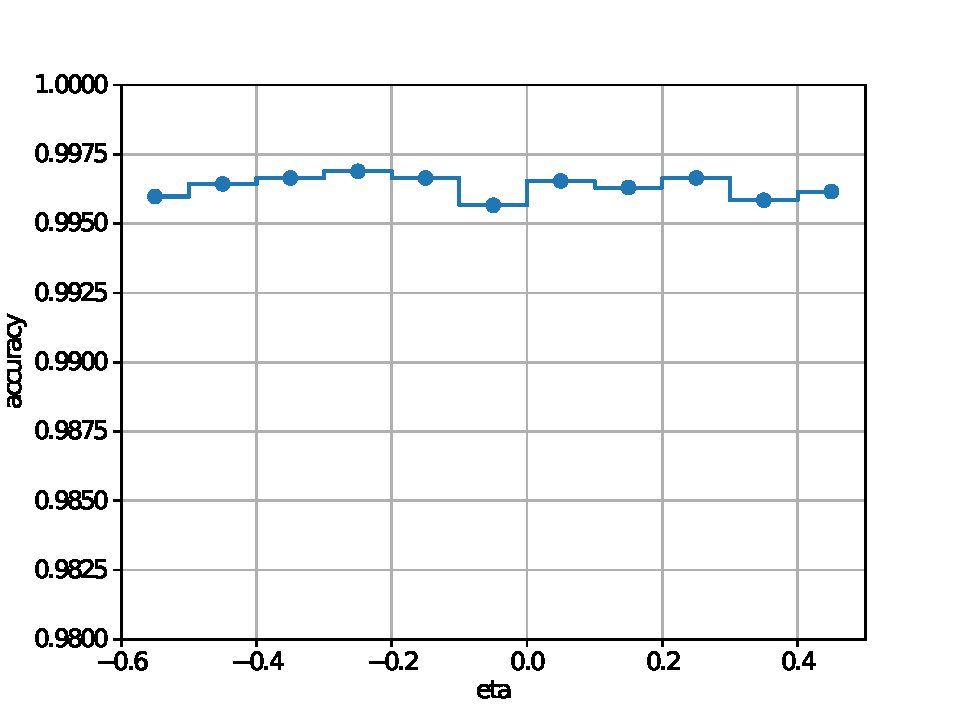
\includegraphics[width=0.45\textwidth]{images/ele_chpi_accuracy_eta_bins.pdf}
\caption{Classification accuracy of best performing network for $\gamma$ vs. $\pi^0$ (top) and $e$ vs. $\pi^\pm$ (bottom), in bins of energy (left) and $\eta$ (right).}
\label{fig:accuracy_bins}
\end{figure*}


%%%% REGRESSION
\subsubsection{Regression Performance}
\label{sec:regression}

Figure~\ref{fig:reg_dnn_vs_cnn_variable} shows the energy regression performance for each particle type, obtained from the end-to-end reconstruction architectures. In this case, we compare against a linear regression algorithm and a BDT (labelled as "XGBoost") representing the current state-of-the-art, as described in Appendix~\ref{app:regression_baseline}. 

\begin{figure*}[htbp]
\centering
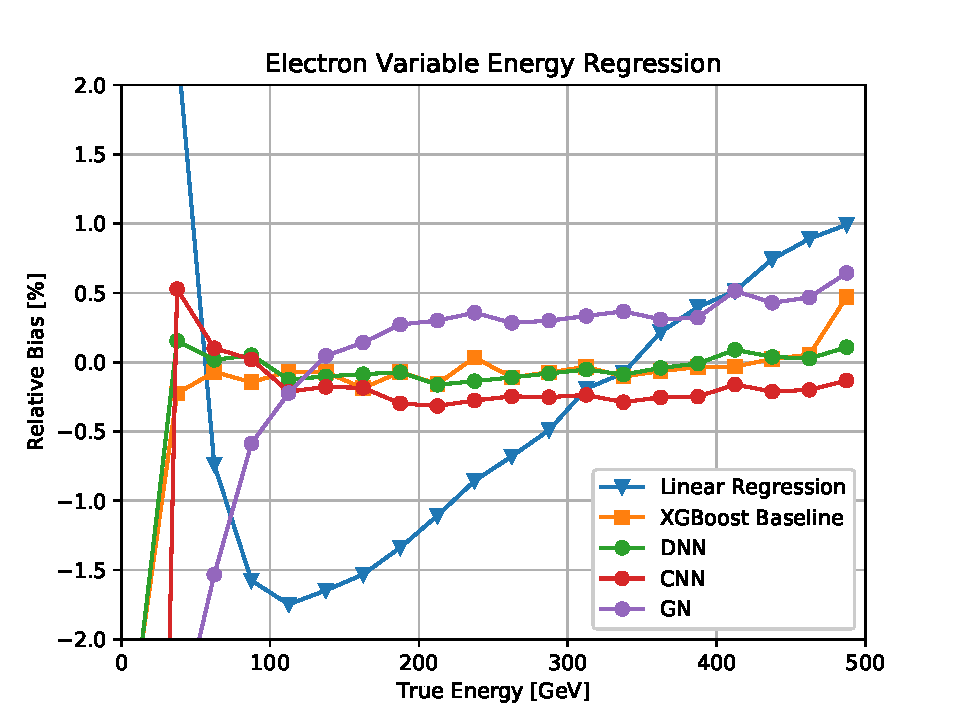
\includegraphics[width=0.38\textwidth]{images/bias_vs_E_Ele_variable}
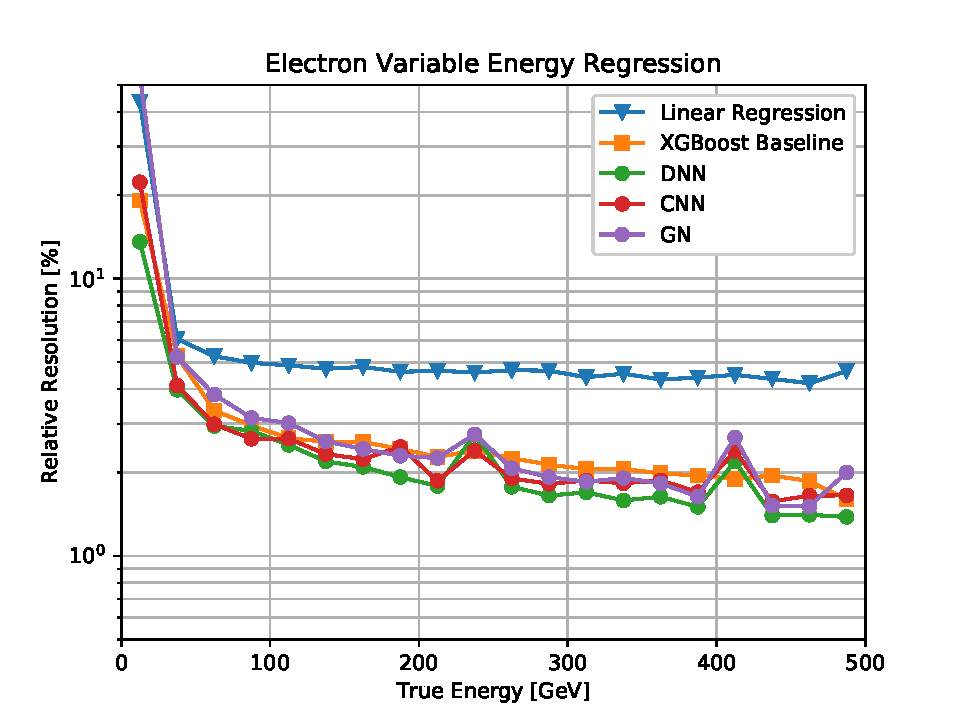
\includegraphics[width=0.38\textwidth]{images/res_vs_E_Ele_variable} \\
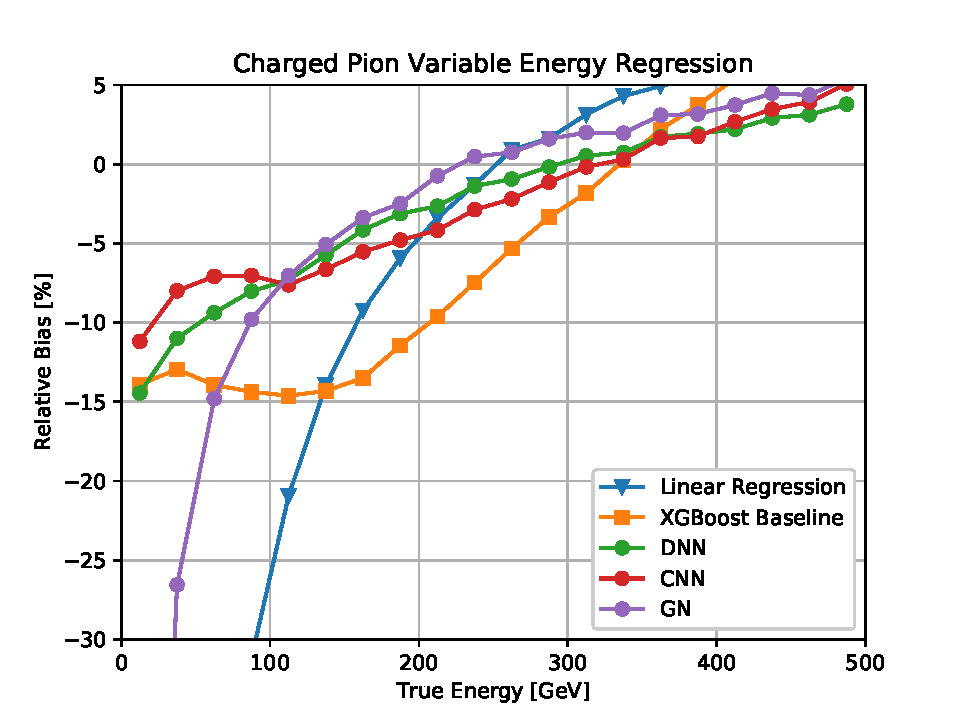
\includegraphics[width=0.38\textwidth]{images/bias_vs_E_ChPi_variable}
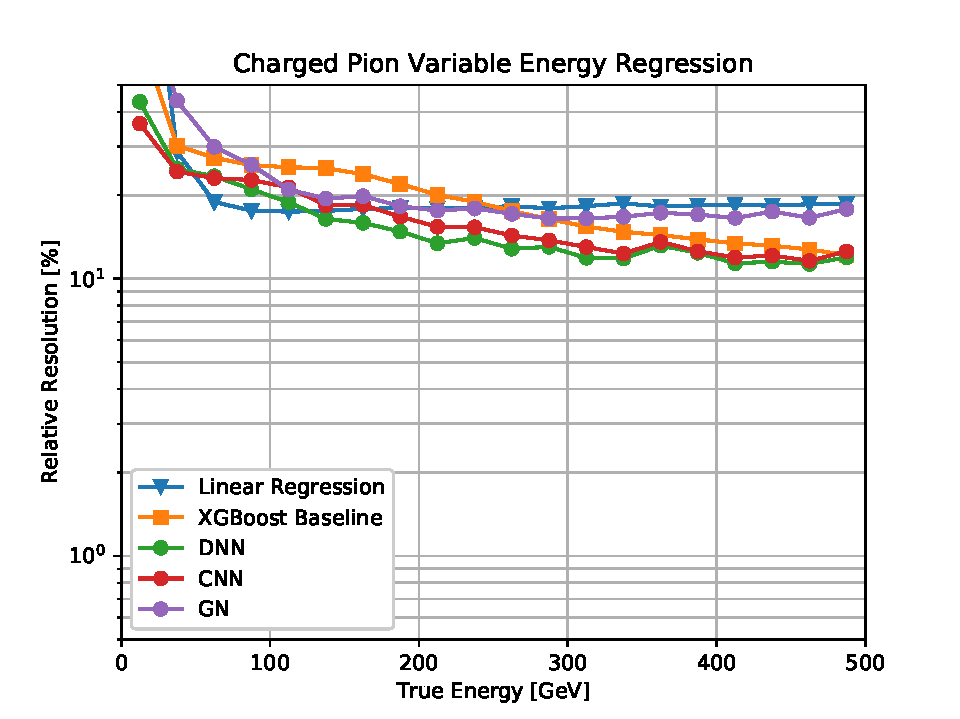
\includegraphics[width=0.38\textwidth]{images/res_vs_E_ChPi_variable}\\
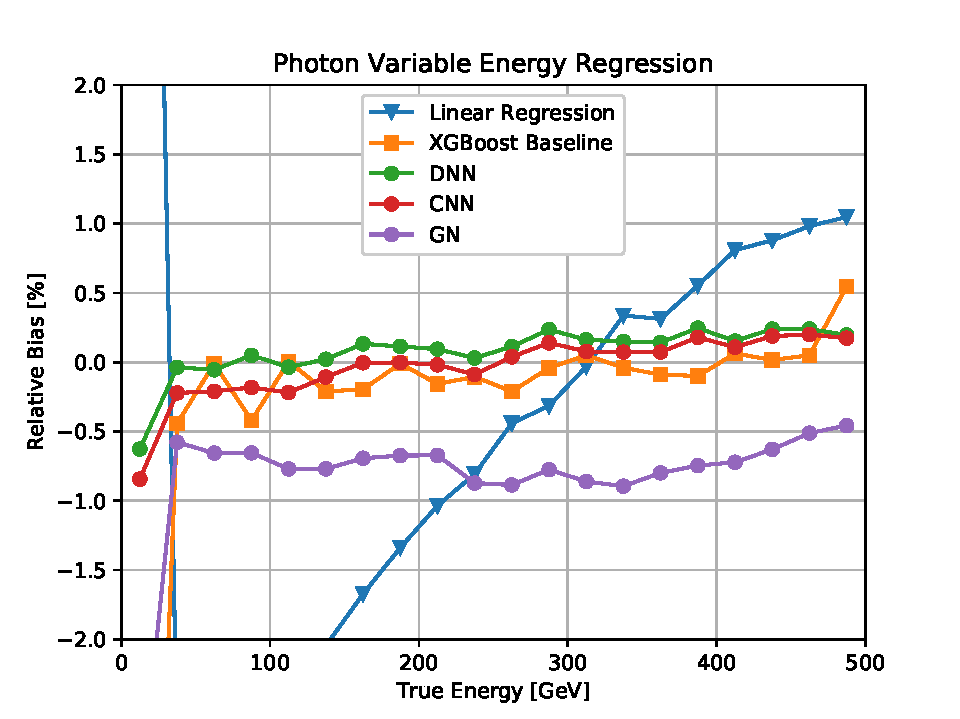
\includegraphics[width=0.38\textwidth]{images/bias_vs_E_Gamma_variable}
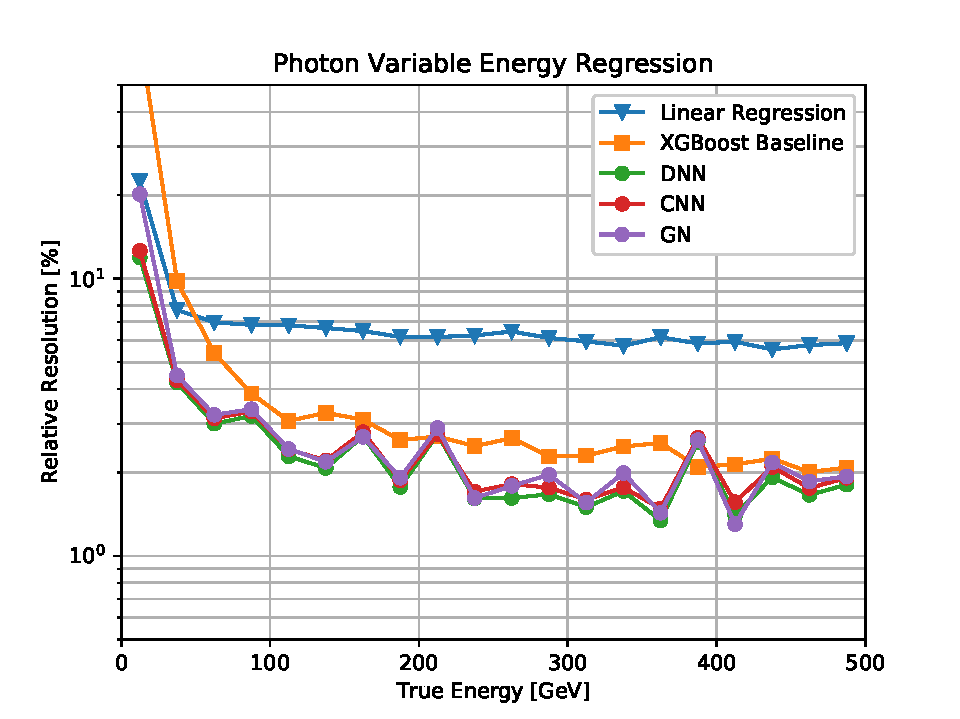
\includegraphics[width=0.38\textwidth]{images/res_vs_E_Gamma_variable}\\
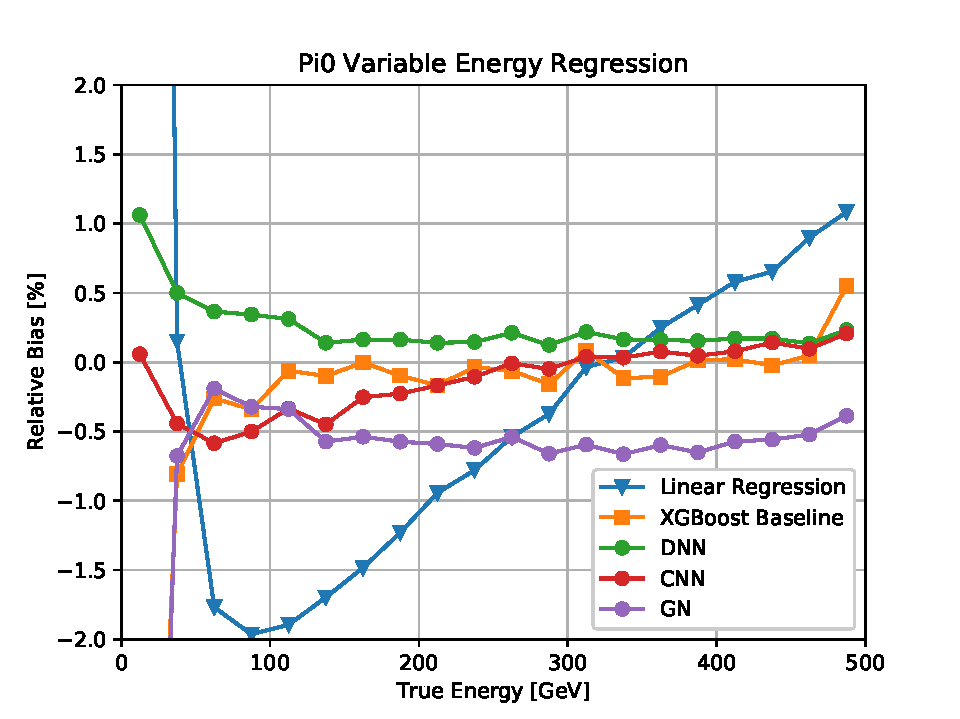
\includegraphics[width=0.38\textwidth]{images/bias_vs_E_Pi0_variable}
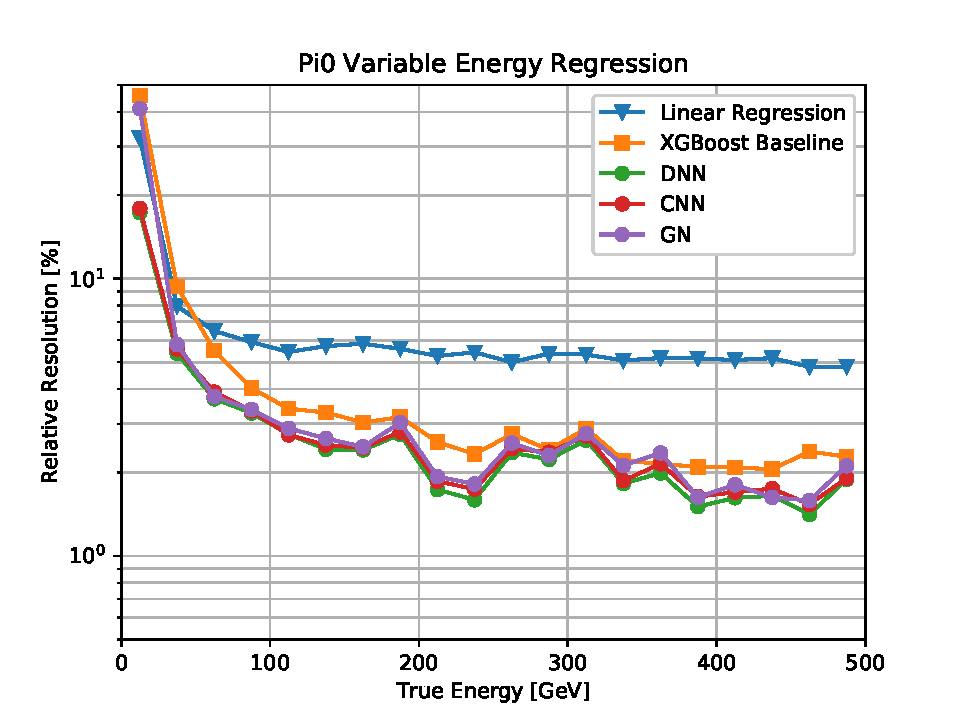
\includegraphics[width=0.38\textwidth]{images/res_vs_E_Pi0_variable}
\caption{Regression bias (left) and resolution (right) as a function
  of true energy for energy predictions on the REC dataset with
  variable-angle incident angle. From top to bottom: electrons,
  charged pions, photons, and neutral
  pions. Algorithms compared are linear regression, XGBoost (BDT), DNN, CNN, and GoogLeNet (GN).\label{fig:reg_dnn_vs_cnn_variable}}
\end{figure*}

Since the energy regression problem is not as complex as the classification problem, the three architectures (DNN, CNN, GN) perform fairly similarly, with the exception of the GN performance on \chpi, which is a bit worse.
%(and possibly slightly over-trained). 
The performance is overall worse for \chpi, both with the networks and with the benchmark baselines (linear regression and XGBoost).

A closer look at the performance boost given by each network can be obtained examining the case of particles entering the calorimeter inner surface at $90^{\mathrm o}$, i.e. with $\eta=0$~\footnote{For these additional fixed-angle regression plots, we did not train GoogLeNet architectures.}. In this case, the problem is more constrained and both the networks and the baseline algorithms are able to perform accurately. The results for fixed angle samples are shown in Appendix~\ref{app:regression_fixed_angle}.

We have also tested the result of training on one class of particle and performing regression on another. These results can be seen in Appendix~\ref{app:xtrain_regression}. In addition, we have looked at the effect on energy regression of increasing the ECAL and HCAL window sizes. This can be seen in Appendix~\ref{app:large_window_regression}.

\subsection{Resampling to ATLAS and CMS Geometries}\label{sec:resampling}

In addition to the results presented so far, we show in this section how the end-to-end reconstruction would perform on calorimeters with granularity and geometry similar to those of the ATLAS and CMS calorimeters. Since the REC dataset (see Section~\ref{sec:data}) is generated using the geometry of the proposed LCD detector, it has a much higher granularity than the current-generation ATLAS and CMS detectors. To visualize how our calorimeter data would look with a coarser detector, we linearly extrapolate the contents of each event to a different calorimeter geometry, using a process we have termed "resampling". To keep the resampling procedure simple, we discard the HCAL information and consider only the ECAL 3D array.

\begin{table*}[tbp]
\centering
\caption{Detailed description of the three detector geometries used in this study: the baseline CLIC ECAL~\cite{CLIC_geometry} and the ATLAS~\cite{Aad:2008zzm} and CMS~\cite{Chatrchyan:2008aa} ECALs.\label{tab:resampling_geometry}}
\begin{tabular}{c|c|ccc|c}
\hline
\multirow{2}{*}{Parameter} & \multirow{2}{*}{\textbf{CLIC}} & \multicolumn{3}{c|}{\textbf{ATLAS}} & \multirow{2}{*}{\textbf{CMS}} \\
            &               & 1st layer & 2nd layer & 3rd layer & \\
\hline
$\Delta \eta$         & 0.003  & 0.025 /8 & 0.025 & 0.5   & 0.0175 \\
$\Delta \phi$         & 0.003  & 0.1      & 0.025 & 0.025 & 0.0175 \\
Radiation Length [cm] & 0.3504 & 14       & 14    & 14    & 0.8903 \\
Moliere radios [cm]   & 0.9327 & 9.043    & 9.043 & 9.043 & 1.959  \\
\hline 
\end{tabular}
\end{table*}

A not-to-scale example of the full procedure is shown in Figure~\ref{fig:resampling}. In this example, we resample the input to a regular square grid with lower granularity than the input data. The operation is simplified in the figure, in order to make the explanation easy to visualize. The actual ATLAS and CMS calorimeter geometries are more complex than a regular array, as described in Table~\ref{tab:resampling_geometry}.

In the resampling process, we first extrapolate each energy value from the grid of CLIC cells to a different geometry. To do so, we scale the content of each CLIC cell to the fraction of overlap area between the CLIC cell and the cell of the target geometry. When computing the overlap fraction, we take into account the fact that different materials have different properties (Moliere radius, interaction length, and radiation length). For instance, CLIC is more fine-grained than CMS or ATLAS detectors, but the Moliere radius of the CLIC ECAL is much smaller than in either of those detectors. This difference determines an offset in the fine binning. Thus, when applying our resampling procedure we normalize the cell size by the detector properties. The Moliere radius is used for $x$ and $y$ re-binning, and radiation length is used for the $z$ direction. At this point we have a good approximation for how the event would look in a calorimeter with the target geometry.

To complete the resampling process, we invert the procedure to go back to our original high-granularity geometry. This last step allows us to keep using the model architectures that we have already optimized. It adds no additional information that would not be present in the low-granularity geometry. This up-sampling also allows us to deal with the irregular geometry of the ATLAS calorimeter by turning it into a neat grid. With no up-sampling, it would not be possible to apply the CNN and GN models. This procedure was validated by comparing total energies before and after resampling, and by visually comparing resampled grids. The energy matches for events were not exact, due to losses at the edge of the resampling grid, and the shower resolutions became much less granular after resampling, but overall the energies and distributions matched before and after the procedure was applied.

\begin{figure}[htbp]
    \centering
    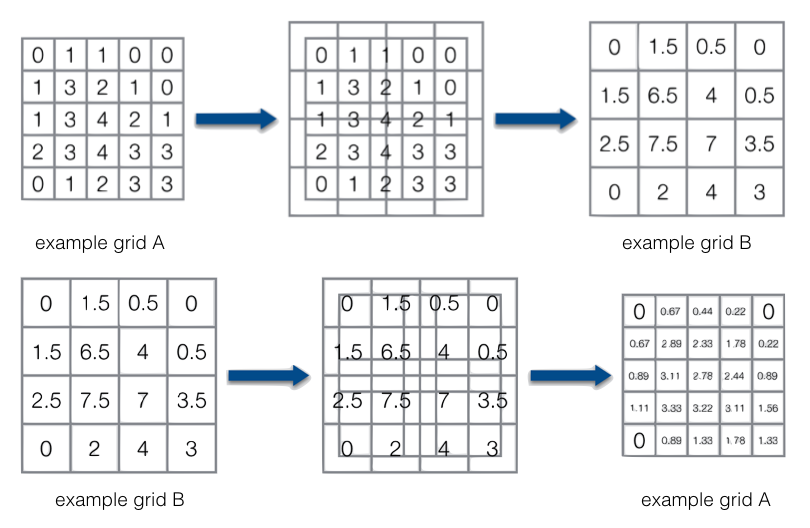
\includegraphics[scale=0.3, clip]{images/resampling.png}
    \caption{Example of the resampling procedure used to emulate CLIC data on a different detector geometry (the example shown here is simply a larger grid). First, we extrapolate hit information from one geometry to another (top). Next, we extrapolate back to the original geometry (bottom). This allows us to emulate the rougher granularity of the second geometry, while keeping data array sizes constant and enabling us to use the models we have already developed for the CLIC dataset. Note that some information is lost at the edges.}
    \label{fig:resampling}
\end{figure}

%\begin{center}
%\begin{tabular}{ l | c c c c c }
% Detector & Cell Size ($\Delta\eta\times\Delta\phi$) & Image Size & Material & $\Chi_0$ [cm] & $R_M$ [cm] \\ 
%\hline
%CLIC          & $0.003\times0.003$     & $25\times25\times25$ & tungsten & 0.35 & 0.92       \\
%CMS           & $0.0175\times0.0175$   & $5\times5\times1$    & lead tungstate & 0.89 & 1.96 \\  
%ATLAS layer 1 & $0.003\times0.1$       & & & & \\
%\caption{Calorimeter properties for the three detector geometries considered. UPDATE FORMAT TO FIT IN ONE COLUMN AND ADD ATLAS 3 LAYERS}
%\end{tabular}
%\end{center}

The resampling procedure comes with a substantial simplification of the underlying physics process. First of all, the information at the edge of the grid is imperfectly translated during the resampling process, leading to worse performance than what could theoretically be achieved in the actual CMS and ATLAS detectors. Also, this simple geometrical rescaling doesn't capture many other detector characteristics. For example, the CMS ECAL detector has no depth information, but being homogeneous it provides a very precise energy measurement. Our resampling method only captures geometric effects, and would not be able to model the improvement in energy resolution. Furthermore, we are unable to include second-order effects such as gaps in the detector geometries. Despite these limitations, one can still extract useful information from the resampled datasets, comparing the classification and regression performances of the end-to-end models defined in Sections~\ref{sec:classification} and~\ref{sec:regression} on different detector geometries.

Comparisons of classification ROC curves between network architectures and our BDT baseline are shown in Figure~\ref{fig:class_ROC_ATLAS_CMS} for ATLAS-like and CMS-like geometries. Here we can see that the previously observed performance ranking still holds true. The GN
model performs best, followed by the CNN, then the DNN. All three networks outperform the BDT baseline. The effect is less pronounced after the CMS-like resampling, due to the low granularity and the single detector layer in the z direction.

\begin{figure}[htbp]
    \centering
    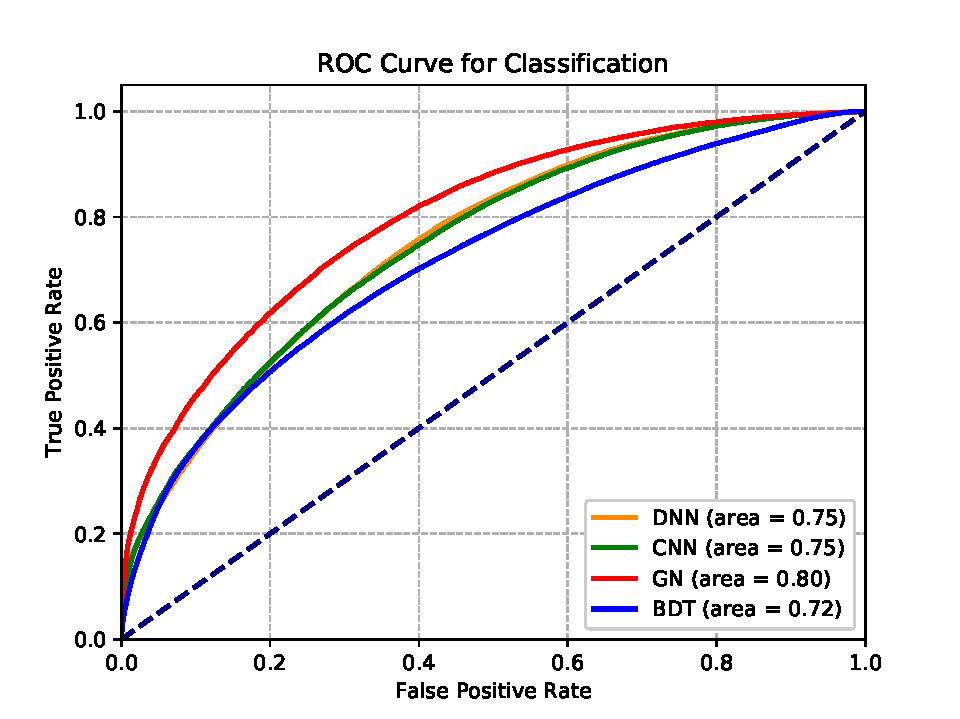
\includegraphics[scale=0.5, clip]{images/classification_ROC_ATLAS}
    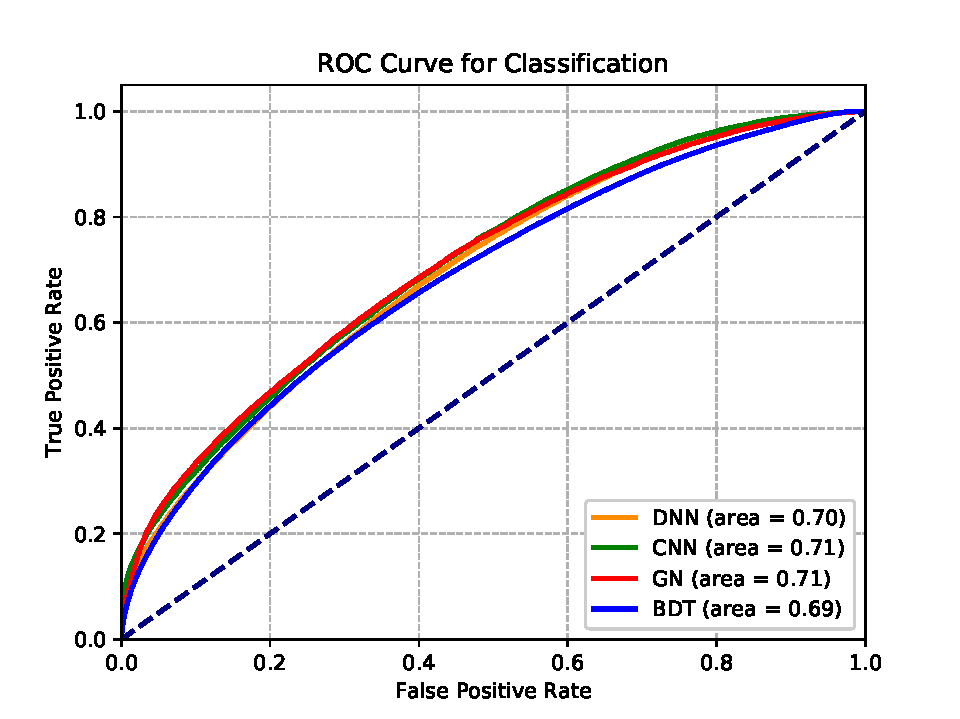
\includegraphics[scale=0.5, clip]{images/classification_ROC_CMS}
    \caption{ROC curve comparisons for variable-angle $\gamma$/$\pi^0$ classification on data resampled to ATLAS-like (top) and CMS-like (bottom) geometries. Algorithms compared are DNN, CNN, GoogLeNet (GN), and BDT.}
    \label{fig:class_ROC_ATLAS_CMS}
\end{figure}

Regression results are shown in Figure~\ref{fig:reg_resampled_gamma_ATLAS_CMS} and~\ref{fig:reg_resampled_pi0_ATLAS_CMS}, for photons and neutral pions (we did not train electrons or charged pions for this comparison). Here we have included the regression baselines, DNN networks, and CNN networks, but not GN (which we did not train on resampled data). The results obtained for the ATLAS-like resampling match those on the REC dataset, with DNN and CNN matching the BDT outcome in terms of bias and surpassing it in resolution. With the CMS-like resampling the neural networks match but do not improves over the BDT energy regression resolution. Once again, this is due to the low spatial resolution in the CMS-like geometry, especially due to the lack of $z$ segmentation. We are unable to model the improved energy resolution from the actual CMS detector, so these energy regression results are based on geometry only.

\begin{figure*}[htbp]
\centering
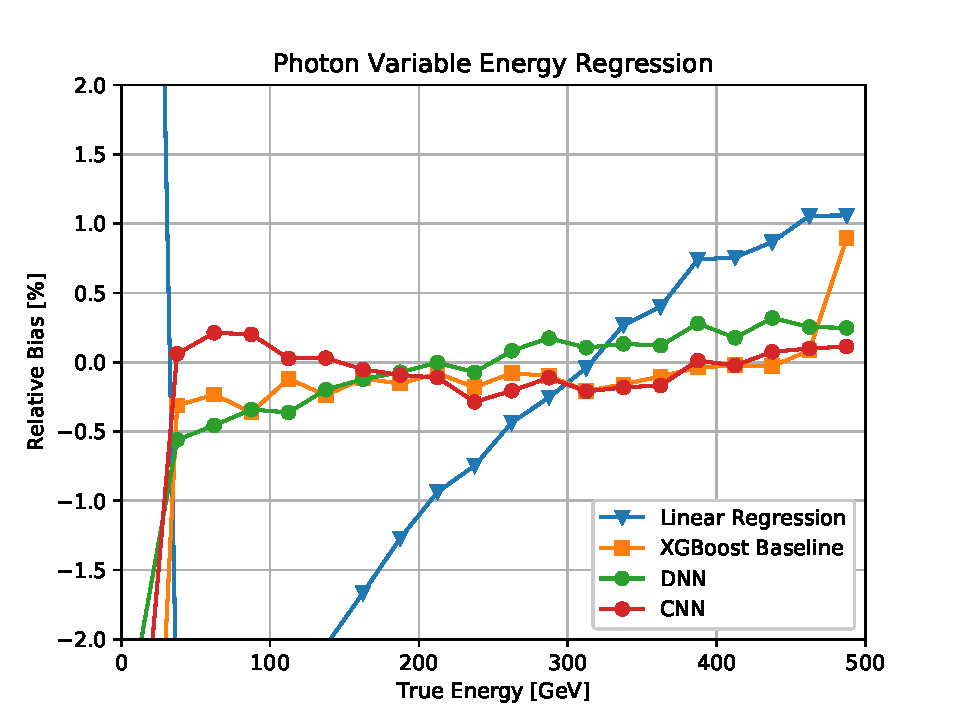
\includegraphics[width=0.38\textwidth]{images/bias_vs_E_Gamma_variable_ATLAS}
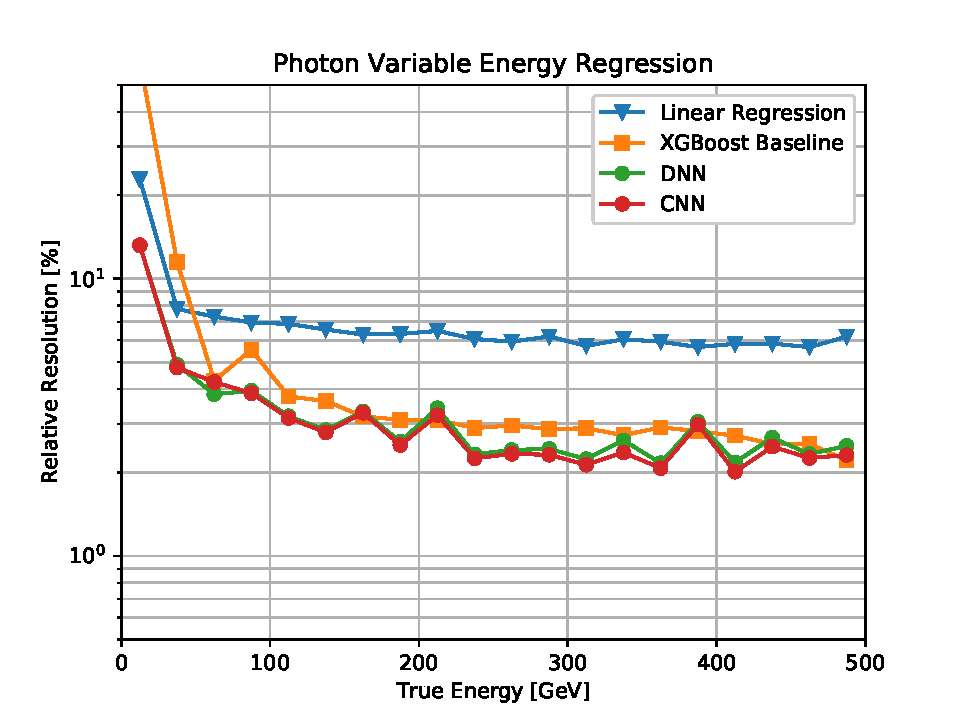
\includegraphics[width=0.38\textwidth]{images/res_vs_E_Gamma_variable_ATLAS} \\
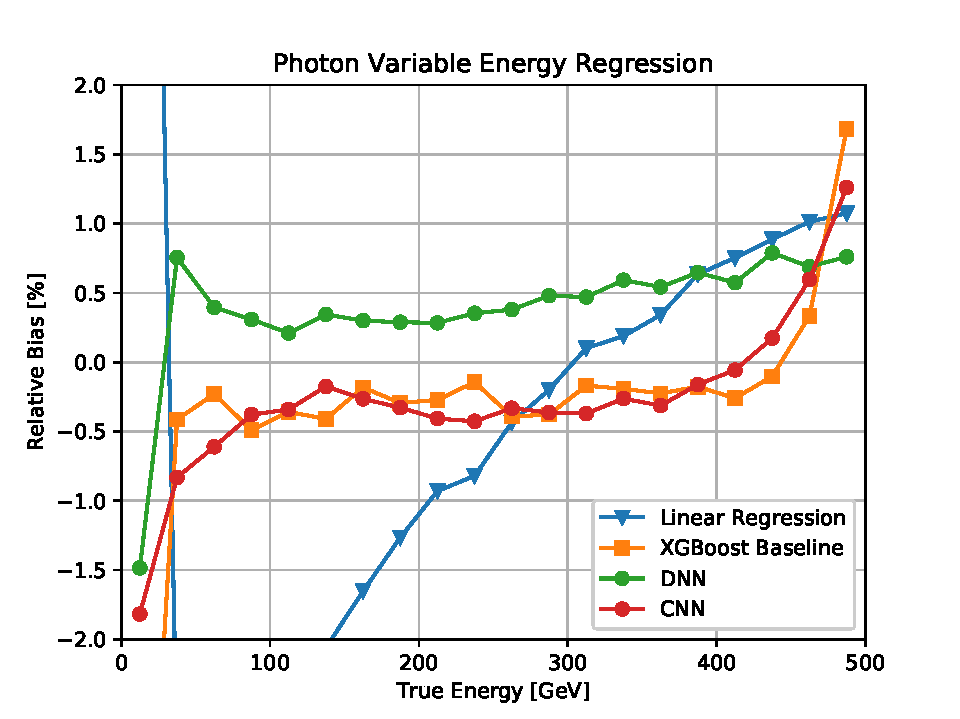
\includegraphics[width=0.38\textwidth]{images/bias_vs_E_Gamma_variable_CMS}
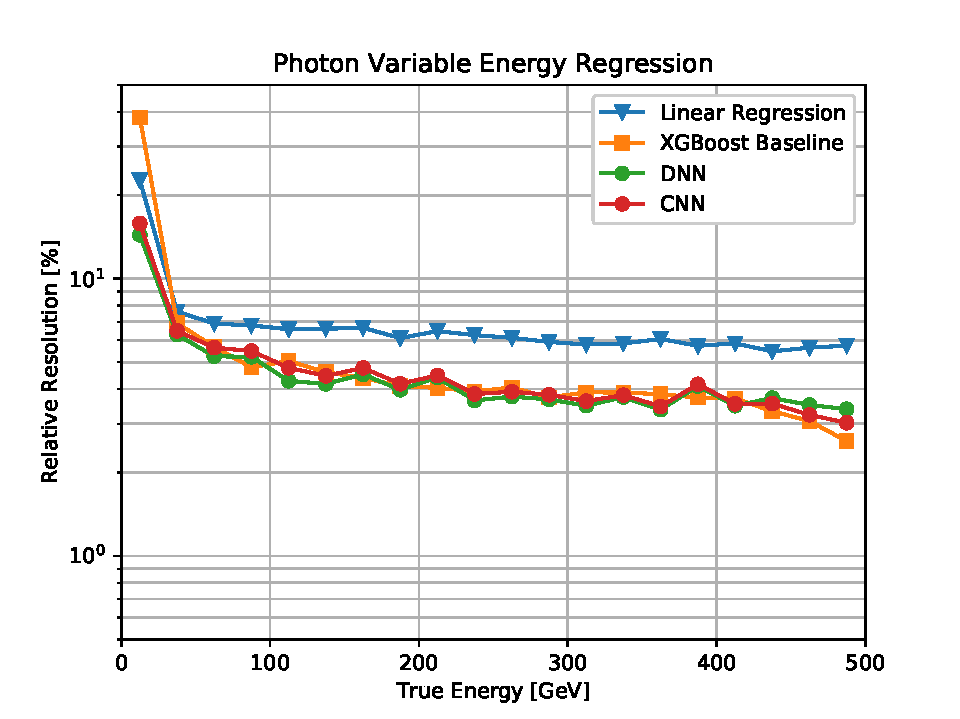
\includegraphics[width=0.38\textwidth]{images/res_vs_E_Gamma_variable_CMS}
\caption{Bias (left) and resolution (right) as a function of true energy for energy predictions for photons, on variable-angle samples resampled to ATLAS-like (top) and CMS-like (bottom) geometries. \label{fig:reg_resampled_gamma_ATLAS_CMS}}
\end{figure*}

\begin{figure*}[htbp]
\centering
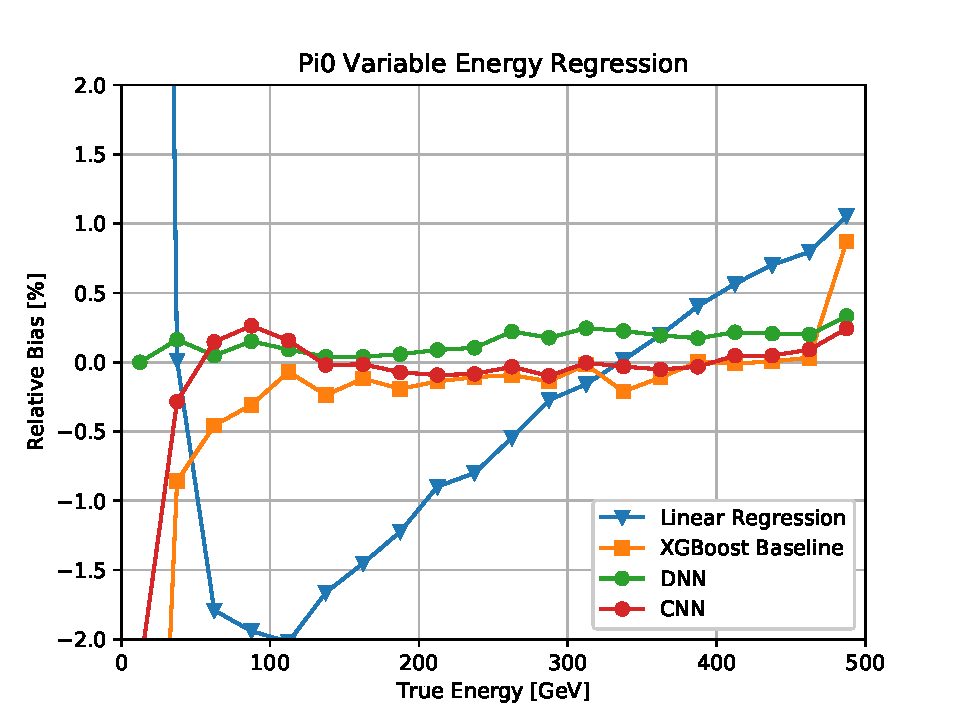
\includegraphics[width=0.38\textwidth]{images/bias_vs_E_Pi0_variable_ATLAS}
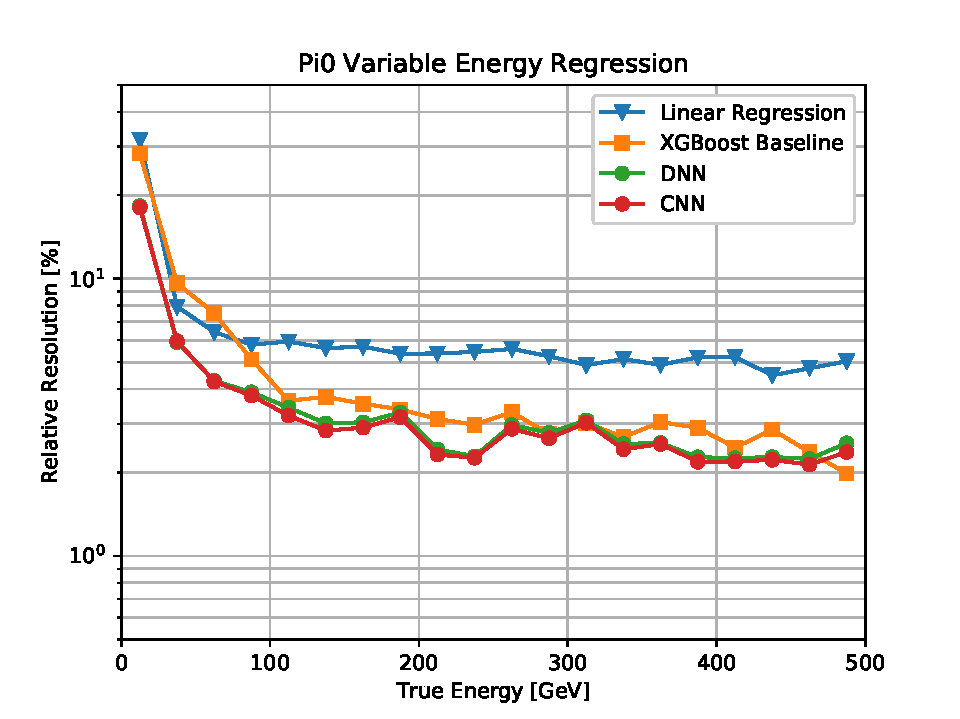
\includegraphics[width=0.38\textwidth]{images/res_vs_E_Pi0_variable_ATLAS} \\
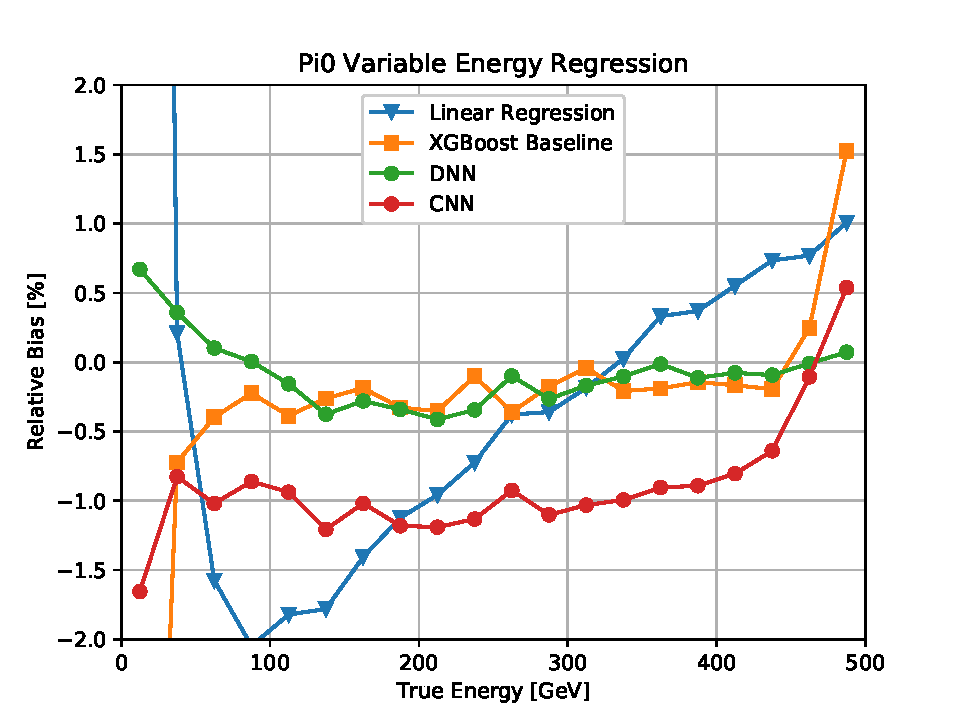
\includegraphics[width=0.38\textwidth]{images/bias_vs_E_Pi0_variable_CMS}
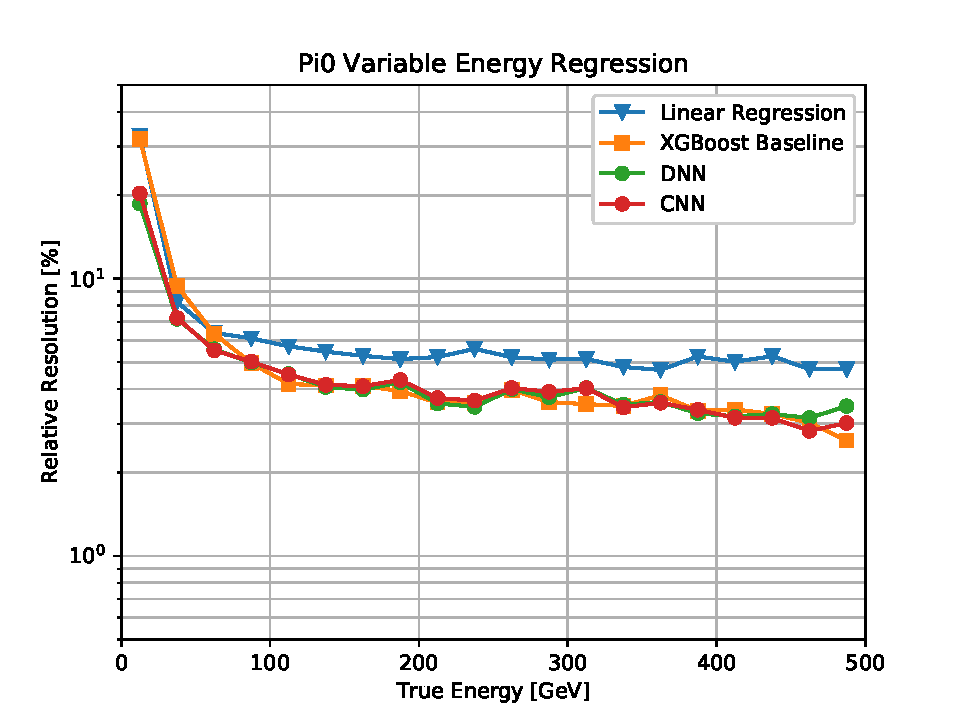
\includegraphics[width=0.38\textwidth]{images/res_vs_E_Pi0_variable_CMS}
\caption{Bias (left) and resolution (right) as a function of true energy for energy predictions for \pizero, on variable-angle samples resampled to  ATLAS-like (top) and CMS-like (bottom) geometries.\label{fig:reg_resampled_pi0_ATLAS_CMS}}
\end{figure*}